\documentclass[edeposit,fullpage,12pt]{uiucthesis2009}
% Use draftthesis for notes and date markings on every page.  Useful when you
%   have multiple copies floating around.
% Use offcenter for the extra .5 inch on the left side. Needed with fullpage and fancy.
% Use mixcasechap for compatibility with hyperref package, which does NOT like all caps default
% Use edeposit for the adviser/committee on the title page.
% Use tocnosub to suppress subsection and lower entries in the TOC.
% PhD candidates use "proquest" for the proquest abstract.

\makeatletter
\DeclareUnicodeCharacter{00A0}{ }
\usepackage{setspace}
\usepackage{graphicx}  % another package that works for figures
\usepackage{multirow}
\usepackage{placeins}
\usepackage{caption}  % allows center figures caption
\usepackage{booktabs} % nice rules (thick lines) for tables
\usepackage{array}
\usepackage{tabularx}
\usepackage[table]{xcolor}
\graphicspath{{figures/}}
\usepackage{amsmath}  % for math spacing
\usepackage{lscape}  % Useful for wide tables or figures.
\usepackage[justification=raggedright]{caption}	% makes captions ragged right - thanks to Bryce Lobdell
\usepackage[acronym,toc]{glossaries}  % acronyms inclusion
\usepackage{color,soul}
\makeglossary
\usepackage{xspace}
\usepackage{float}
\usepackage{subcaption}
\usepackage{amsmath}%
\allowdisplaybreaks
\usepackage{MnSymbol}%
\usepackage{wasysym}%
\usepackage{adjustbox}
\usepackage{enumitem}
\usepackage{tkz-euclide}
\usepackage{tikz}
\usetikzlibrary{positioning, arrows, decorations, shapes}
\usetikzlibrary{shapes.geometric,arrows}
\def\checkmark{\tikz\fill[scale=0.4](0,.35) -- (.25,0) -- (1,.7) -- (.25,.15) -- cycle;} 

\definecolor{illiniblue}{HTML}{B1C6E2}
\definecolor{illiniorange}{HTML}{f8c2a2}
\definecolor{fhrblue}{HTML}{0000ff}
\definecolor{fhrgrey}{HTML}{808080}
\definecolor{fhrblack}{HTML}{040404}
\definecolor{fhrred}{HTML}{f10a0a}
\definecolor{fhrgreen}{HTML}{2f6d39}
\definecolor{fhryellow}{HTML}{fdfe36}
\definecolor{fhrpink}{HTML}{ffb8c5}
\definecolor{fhrorange}{HTML}{ffa500}
\definecolor{fhrpurple}{HTML}{800080}
\definecolor{pink}{HTML}{e2b1c2}
\definecolor{green}{HTML}{c2e2b1}
\definecolor{purple}{HTML}{b9b1e2}
\definecolor{fhrblue1}{HTML}{0000bd}
\definecolor{fhrblue2}{HTML}{0283bd}
\definecolor{fhrblue3}{HTML}{0042bd}
\definecolor{fhrred1}{HTML}{c80100}
\definecolor{fhrblack1}{HTML}{000000}
\definecolor{fhrwhite1}{HTML}{c7c5bd}
\definecolor{fhrgrey1}{HTML}{82807a}
\tikzstyle{loblock} = [rectangle, draw, fill=illiniorange, 
text width=15em, text centered, rounded corners, minimum height=3em]
\tikzstyle{lbblock} = [rectangle, draw, fill=illiniblue, 
text width=15em, text centered, rounded corners, minimum height=3em]
\tikzstyle{oblock} = [rectangle, draw, fill=illiniorange, 
text width=10em, text centered, rounded corners, minimum height=3em]
\tikzstyle{bblock} = [rectangle, draw, fill=illiniblue, 
text width=10em, text centered, rounded corners, minimum height=3em]
\tikzstyle{arrow} = [thick,->,>=stealth]
\tikzstyle{bbblock} = [rectangle, draw, fill=illiniblue, 
text width=1em, text centered, rounded corners, minimum height=1em]
\tikzstyle{boblock} = [rectangle, draw, fill=illiniorange, 
text width=1em, text centered, rounded corners, minimum height=1em]
\tikzstyle{e72block} = [rectangle, fill=none, 
text width=7.3em, text centered, rounded corners, minimum height=2em]
\tikzstyle{o72block} = [rectangle, draw, fill=illiniorange, 
text width=7.3em, text centered, rounded corners, minimum height=2em]
\tikzstyle{b72block} = [rectangle, draw, fill=illiniblue, 
text width=7.3em, text centered, rounded corners, minimum height=2em]
\tikzstyle{e82block} = [rectangle, fill=none, 
text width=8.3em, text centered, rounded corners, minimum height=2em]
\tikzstyle{b82block} = [rectangle, draw, fill=illiniblue, 
text width=8em, text centered, rounded corners, minimum height=2em]
\tikzstyle{b223block} = [rectangle, draw, fill=illiniblue, 
text width=22em, text centered, rounded corners, minimum height=3em]
\usepackage[document]{ragged2e}
\usepackage{booktabs}% http://ctan.org/pkg/booktabs
\newcommand{\tabitem}{~~\llap{\textbullet}~~}
\usepackage{hyperref}
\hypersetup{hidelinks}
\usepackage{minted}

\phdthesis

\title{Fluoride-Salt-Cooled High-Temperature Reactor Design Optimization with Evolutionary Algorithms}
\author{Gwendolyn J.Y. Chee}
\department{Nuclear, Plasma, and Radiological Engineering}
\degreeyear{2022}

% Advisor name is required for
% - doctoral students for the ProQuest abstract
% - master's students who do not have a master's committee
%\advisor{Professor Kathryn D. Huff}

\committee{Associate Professor Kathryn D. Huff, Chair \\
           Research Scientist Madicken Munk \\
           Associate Professor Tomasz Kozlowski \\
           Professor James F. Stubbins \\
           Research Assistant Professor Huy Trong Tran} 

\begin{document}
%\newacronym{<++>}{<++>}{<++>}
\newacronym[longplural={metric tons of heavy metal}]{MTHM}{MTHM}{metric ton of heavy metal}
\newacronym{3D CAD}{3D CAD}{three-dimensional Computer-Aided Design}
\newacronym{AHTR}{AHTR}{Advanced High-Temperature Reactor}
\newacronym{AI}{AI}{artificial intelligence}
\newacronym{AMAFT}{AMAFT}{Additive Manufacturing as an Alternative Fabrication Technique}
\newacronym{ANDRA}{ANDRA}{Agence Nationale pour la gestion des D\'echets RAdioactifs, the French National Agency for Radioactive Waste Management}
\newacronym{ANL}{ANL}{Argonne National Laboratory}
\newacronym{ANS}{ANS}{American Nuclear Society}
\newacronym{API}{API}{application programming interface}
\newacronym{ARE}{ARE}{Aircraft Reactor Experiment}
\newacronym{ARFC}{ARFC}{Advanced Reactors and Fuel Cycles}
\newacronym{BP}{BP}{burnable poison}
\newacronym{CFD}{CFD}{Computational Fluid Dynamics}
\newacronym{CEA}{CEA}{Commissariat \`a l'\'Energie Atomique et aux \'Energies Alternatives}
\newacronym{CI}{CI}{continuous integration}
\newacronym{CIEMAT}{CIEMAT}{Centro de Investigaciones Energéticas, Medioambientales y Tecnológicas}
\newacronym{CNEN}{CNEN}{Comiss\~{a}o Nacional de Energia Nuclear}
\newacronym{CNERG}{CNERG}{Computational Nuclear Engineering Research Group}
\newacronym{CNRS}{CNRS}{Le Centre National De La Recherche Scientifique}
\newacronym{COSI}{COSI}{Commelini-Sicard}
\newacronym{COTS}{COTS}{commercial, off-the-shelf}
\newacronym{CR}{CR}{control rod}
\newacronym{CSNF}{CSNF}{commercial spent nuclear fuel}
\newacronym{CTAH}{CTAHs}{Coiled Tube Air Heaters}
\newacronym{CUBIT}{CUBIT}{CUBIT Geometry and Mesh Generation Toolkit}
\newacronym{CURIE}{CURIE}{Centralized Used Fuel Resource for Information Exchange}
\newacronym{CVI}{CVI}{chemical vapor infiltration}
\newacronym{CZP}{CZP}{cold zero power}
\newacronym{DEAP}{DEAP}{Distributed Evolutionary Algorithms in Python}
\newacronym{DESAE}{DESAE}{Dynamic Analysis of Nuclear Energy Systems Strategies}
\newacronym{DNBR}{DNBR}{Departure from nucleate boiling ratio}
\newacronym{DNP}{DNP}{delayed neutron precursor}
\newacronym{DOE}{DOE}{Department of Energy}
\newacronym{dpa}{dpa}{displacements per atom}
\newacronym{DRACS}{DRACS}{Direct Reactor Auxiliary Cooling System}
\newacronym{DRE}{DRE}{dynamic resource exchange}
\newacronym{DSNF}{DSNF}{DOE spent nuclear fuel}
\newacronym{DYMOND}{DYMOND}{Dynamic Model of Nuclear Development }
\newacronym{EA}{EA}{evolutionary algorithm}
\newacronym{EBM}{EBM}{electron beam melting}
\newacronym{EBS}{EBS}{Engineered Barrier System}
\newacronym{EDF}{EDF}{Électricité de France}
\newacronym{EDZ}{EDZ}{Excavation Disturbed Zone}
\newacronym{EG}{EG}{Evaluation Group}
\newacronym{EIA}{EIA}{U.S. Energy Information Administration}
\newacronym{EPA}{EPA}{Environmental Protection Agency}
\newacronym{EPR}{EPR}{European Pressurized Reactors}
\newacronym{EPRI}{EPRI}{Electric Power Research Institute}
\newacronym{EP}{EP}{Engineering Physics}
\newacronym{EU}{EU}{European Union}
\newacronym{FCM}{FCM}{fully ceramic microencapsulated}
\newacronym{FCO}{FCO}{Fuel Cycle Options}
\newacronym{FCT}{FCT}{Fuel Cycle Technology}
\newacronym{FD}{FD}{fission density}
\newacronym{FEHM}{FEHM}{Finite Element Heat and Mass Transfer}
\newacronym{FEPs}{FEPs}{Features, Events, and Processes}
\newacronym{FHR}{FHR}{Fluoride-Salt-Cooled High-Temperature Reactor}
\newacronym{FLiBe}{FLiBe}{Fluoride-Lithium-Beryllium}
\newacronym{FM}{FM}{ferritic/martensitic}
\newacronym{FP}{FP}{Fission Product}
\newacronym{GA}{GA}{genetic algorithm}
\newacronym{GDSE}{GDSE}{Generic Disposal System Environment}
\newacronym{GDSM}{GDSM}{Generic Disposal System Model}
\newacronym{Georgia Tech}{Georgia Tech}{Georgia Institute of Technology}
\newacronym{GENIUSv1}{GENIUSv1}{Global Evaluation of Nuclear Infrastructure Utilization Scenarios, Version 1}
\newacronym{GENIUSv2}{GENIUSv2}{Global Evaluation of Nuclear Infrastructure Utilization Scenarios, Version 2}
\newacronym{GENIUS}{GENIUS}{Global Evaluation of Nuclear Infrastructure Utilization Scenarios}
\newacronym{GFR}{GFR}{Gas-Cooled Fast Reactor}
\newacronym{GHG}{GHG}{greenhouse gas}
\newacronym{GIF}{GIF}{Generation IV International Forum}
\newacronym{GUI}{GUI}{graphical user interface}
\newacronym{HEM}{HEM}{Homogenous Equilibrium Mixture}
\newacronym{HFIR}{HFIR}{High Flux Isotope Reactor}
\newacronym{HLW}{HLW}{high level waste}
\newacronym{HM}{HM}{heavy metal}
\newacronym{HPC}{HPC}{high-performance computing}
\newacronym{HTC}{HTC}{high-throughput computing}
\newacronym{HTGR}{HTGR}{High Temperature Gas-Cooled Reactor}
\newacronym{HZP}{HZP}{hot zero power}
\newacronym{IAEA}{IAEA}{International Atomic Energy Agency}
\newacronym{IEMA}{IEMA}{Illinois Emergency Mangament Agency}
\newacronym{IHLRWM}{IHLRWM}{International High Level Radioactive Waste Management}
\newacronym{INL}{INL}{Idaho National Laboratory}
\newacronym{IPRR1}{IRP-R1}{Instituto de Pesquisas Radioativas Reator 1}
\newacronym{IRP}{IRP}{Integrated Research Project}
\newacronym{IRSN}{IRSN}{Institute for Radiological Protection and Nuclear Safety}
\newacronym{ISFSI}{ISFSI}{Independent Spent Fuel Storage Installation}
\newacronym{ISRG}{ISRG}{Independent Student Research Group}
\newacronym{JAEA}{JAEA}{Japanese Atomic Energy Agency}
\newacronym{JFNK}{JFNK}{Jacobian-Free Newton Krylov}
\newacronym{LANL}{LANL}{Los Alamos National Laboratory}
\newacronym{LBNL}{LBNL}{Lawrence Berkeley National Laboratory}
\newacronym{LCOE}{LCOE}{levelized cost of electricity}
\newacronym{L-DED}{L-DED}{laser directed energy deposition}
\newacronym{LDRD}{LDRD}{laboratory directed research and development}
\newacronym{LEU}{LEU}{low-enriched uranium}
\newacronym{LFR}{LFR}{Lead-Cooled Fast Reactor}
\newacronym{LLNL}{LLNL}{Lawrence Livermore National Laboratory}
\newacronym{LMFBR}{LMFBR}{Liquid Metal Fast Breeder Reactor}
\newacronym{LOFC}{LOFC}{Loss of Forced Cooling}
\newacronym{LOHS}{LOHS}{Loss of Heat Sink}
\newacronym{LOLA}{LOLA}{Loss of Large Area}
\newacronym{LP}{LP}{linear program}
\newacronym{LPD}{LPD}{Local power density}
\newacronym{LWR}{LWR}{Light Water Reactor}
\newacronym{MA}{MA}{minor actinide}
\newacronym{MCNP}{MCNP}{Monte Carlo N-Particle code}
\newacronym{MHC}{MHC}{molybdenum–hafnium carbide alloy}
\newacronym{MILP}{MILP}{mixed-integer linear program}
\newacronym{MIT}{MIT}{Massachusetts Institute of Technology}
\newacronym{MOAB}{MOAB}{Mesh-Oriented datABase}
\newacronym{MOOSE}{MOOSE}{Multiphysics Object-Oriented Simulation Environment}
\newacronym{MOSART}{MOSART}{Molten Salt Actinide Recycler and Transmuter}
\newacronym{MOX}{MOX}{mixed oxide}
\newacronym{MPI}{MPI}{Message Passing Interface}
\newacronym{MSBR}{MSBR}{Molten Salt Breeder Reactor}
\newacronym{MSFR}{MSFR}{Molten Salt Fast Reactor}
\newacronym{MSRE}{MSRE}{Molten Salt Reactor Experiment}
\newacronym{MSR}{MSR}{Molten Salt Reactor}
\newacronym{NAGRA}{NAGRA}{National Cooperative for the Disposal of Radioactive Waste}
\newacronym{NEA}{NEA}{Nuclear Energy Agency}
\newacronym{NEM}{NEM}{Nodal Expansion Method}
\newacronym{NEAMS}{NEAMS}{Nuclear Engineering Advanced Modeling and Simulation}
\newacronym{NESTLE}{NESTLE}{Nodal Eigenvalue, Steady-state, Transient, Le core Evaluator}
\newacronym{NEUP}{NEUP}{Nuclear Energy University Programs}
\newacronym{NFC}{NFC}{Nuclear Fuel Cycle}
\newacronym{NFCSim}{NFCSim}{Nuclear Fuel Cycle Simulator}
\newacronym{NGNP}{NGNP}{Next Generation Nuclear Plant}
\newacronym{NMR-50}{NMR-50}{Purdue Novel Modular Reactor}
\newacronym{NMWPC}{NMWPC}{Nuclear MW Per Capita}
\newacronym{NNL}{NNL}{National Nuclear Laboratory}
\newacronym{NNSA}{NNSA}{National Nuclear Security Administration}
\newacronym{NPRE}{NPRE}{Department of Nuclear, Plasma, and Radiological Engineering}
\newacronym{NQA1}{NQA-1}{Nuclear Quality Assurance - 1}
\newacronym{NRC}{NRC}{Nuclear Regulatory Commission}
\newacronym{NSF}{NSF}{National Science Foundation}
\newacronym{NSGA-II}{NSGA-II}{Non-dominated Sorting Genetic Algorithm II}
\newacronym{NSSC}{NSSC}{Nuclear Science and Security Consortium}
\newacronym{NUWASTE}{NUWASTE}{Nuclear Waste Assessment System for Technical Evaluation}
\newacronym{NWF}{NWF}{Nuclear Waste Fund}
\newacronym{NWTRB}{NWTRB}{Nuclear Waste Technical Review Board}
\newacronym{OCRWM}{OCRWM}{Office of Civilian Radioactive Waste Management}
\newacronym{OECD}{OECD}{Organisation for Economic Co-operation and Development}
\newacronym{ORION}{ORION}{ORION}
\newacronym{ORNL}{ORNL}{Oak Ridge National Laboratory}
\newacronym{PARCS}{PARCS}{Purdue Advanced Reactor Core Simulator}
\newacronym{PCA}{PCA}{Particle Collision Algorithm}
\newacronym{PBAHTR}{PB-AHTR}{Pebble Bed Advanced High Temperature Reactor}
\newacronym{PBFHR}{PB-FHR}{Pebble-Bed Fluoride-Salt-Cooled High-Temperature Reactor}
\newacronym{PDE}{PDE}{Partial Differential Equation}
\newacronym{PEI}{PEI}{Peak Environmental Impact}
\newacronym{PH}{PRONGHORN}{PRONGHORN}
\newacronym{PIRT}{PIRT}{Phenomena Identification and Ranking Table}
\newacronym{PPF}{PPF}{Power peaking factor}
\newacronym{PRIS}{PRIS}{Power Reactor Information System}
\newacronym{PRKE}{PRKE}{Point Reactor Kinetics Equations}
\newacronym{PSPG}{PSPG}{Pressure-Stabilizing/Petrov-Galerkin}
\newacronym{PWAR}{PWAR}{Pratt and Whitney Aircraft Reactor}
\newacronym{PWR}{PWR}{Pressurized Water Reactor}
\newacronym{PyNE}{PyNE}{Python toolkit for Nuclear Engineering}
\newacronym{PyRK}{PyRK}{Python for Reactor Kinetics}
\newacronym{PyPI}{PyPI}{The Python Package Index}
\newacronym{QA}{QA}{quality assurance}
\newacronym{RDD}{RD\&D}{Research Development and Demonstration}
\newacronym{RD}{R\&D}{Research and Development}
\newacronym{REALM}{REALM}{Reactor Evolutionary Algorithm Optimizer}
\newacronym{REE}{REE}{rare earth element}
\newacronym{RELAP}{RELAP}{Reactor Excursion and Leak Analysis Program}
\newacronym{RIA}{RIA}{Reactivity Insertion Accident}
\newacronym{RIF}{RIF}{Region-Institution-Facility}
\newacronym{ROLLO}{ROLLO}{Reactor evOLutionary aLgorithm Optimizer}
\newacronym{SA}{SA}{Simulation Annealing}
\newacronym{SCK CEN}{SCK CEN}{Studiecentrum voor Kernenergie}
\newacronym{SCWR}{SCWR}{Supercritical-Water-Cooled Reactor}
\newacronym{SFR}{SFR}{Sodium-Cooled Fast Reactor}
\newacronym{SF-TMSR}{SF-TMSR}{Solid Fuel Thorium Molten Salt Reactor}
\newacronym{SiC}{SiC}{silicon carbide}
\newacronym{SINAP}{SINAP}{Shanghai Institute of Applied Physics}
\newacronym{SINDAG}{SINDA{\textbackslash}G}{Systems Improved Numerical Differencing Analyzer $\backslash$ Gaski}
\newacronym{SKB}{SKB}{Svensk K\"{a}rnbr\"{a}nslehantering AB}
\newacronym{SLM}{SLM}{selective laser melting}
\newacronym{SmAHTR}{SmAHTR}{Small Modular AHTR}
\newacronym{SNF}{SNF}{spent nuclear fuel}
\newacronym{SNL}{SNL}{Sandia National Laboratory}
\newacronym{STC}{STC}{specific temperature change}
\newacronym{SUPG}{SUPG}{Streamline-Upwind/Petrov-Galerkin}
\newacronym{SWF}{SWF}{Separations and Waste Forms}
\newacronym{SWU}{SWU}{Separative Work Unit}
\newacronym{TCR}{TCR}{Transformational Challenge Reactor}
\newacronym{TRIGA}{TRIGA}{Training Research Isotope General Atomic}
\newacronym{TRISO}{TRISO}{Tristructural Isotropic}
\newacronym{TSM}{TSM}{Total System Model}
\newacronym{TSPA}{TSPA}{Total System Performance Assessment for the Yucca Mountain License Application}
\newacronym{ThOX}{ThOX}{thorium oxide}
\newacronym{UCB}{UCB}{University of California Berkeley}
\newacronym{UFD}{UFD}{Used Fuel Disposition}
\newacronym{UML}{UML}{Unified Modeling Language}
\newacronym{UN}{UN}{uranium nitride}
\newacronym{UOX}{UOX}{uranium oxide}
\newacronym{UQ}{UQ}{uncertainty quantification}
\newacronym{US}{US}{United States}
\newacronym{USC}{USC}{University of South Carolina}
\newacronym{UIUC}{UIUC}{University of Illinois at Urbana-Champaign}
\newacronym{UT Austin}{UT Austin}{The University of Texas at Austin}
\newacronym{VHTR}{VHTR}{Very-High-Temperature Reactor}
\newacronym{VV}{V\&V}{verification and validation}
\newacronym{WCT}{WCT}{wall-clock-time}
\newacronym{YMR}{YMR}{Yucca Mountain Repository Site}
%%%%%%%%%%%%%%%%%%%%%%%%%%%%%%%%%%%%%%%%%%%%%%%%%%%%%%%%%%%%%%%%%%%%%%%%%%%%%%%
% TITLE
%
\maketitle
\justify
\parindent 2em%

%\frontmatter
%%%%%%%%%%%%%%%%%%%%%%%%%%%%%%%%%%%%%%%%%%%%%%%%%%%%%%%%%%%%%%%%%%%%%%%%%%%%%%%
% ABSTRACT
%

%\begin{abstract}
%    \input{abs}
%\end{abstract}

%%%%%%%%%%%%%%%%%%%%%%%%%%%%%%%%%%%%%%%%%%%%%%%%%%%%%%%%%%%%%%%%%%%%%%%%%%%%%%%
% TABLE OF CONTENTS
%
\tableofcontents

%%%%%%%%%%%%%%%%%%%%%%%%%%%%%%%%%%%%%%%%%%%%%%%%%%%%%%%%%%%%%%%%%%%%%%%%%%%%%%%
% LIST OF TABLES
%
% The List of Tables is not strictly necessary. Omitting the List of Tables will
% simplify the thesis check and reduce the number of corrections.
%\listoftables

%%%%%%%%%%%%%%%%%%%%%%%%%%%%%%%%%%%%%%%%%%%%%%%%%%%%%%%%%%%%%%%%%%%%%%%%%%%%%%%
% LIST OF FIGURES
%
% The List of Figures is not strictly necessary. Omitting the List of Figures will
% simplify the thesis check and reduce the number of corrections.
%\listoffigures

%%%%%%%%%%%%%%%%%%%%%%%%%%%%%%%%%%%%%%%%%%%%%%%%%%%%%%%%%%%%%%%%%%%%%%%%%%%%%%%
% LIST OF ABBREVIATIONS
%
% The List of Abbreviations is not strictly necessary.
%\chapter{LIST OF ABBREVIATIONS}

%\printacronyms
%\begin{symbollist*}
%\item[MSBR] Molten Salt Breeder Reactor
%\item[MSR] Molten Salt Reactor
%\item[ORNL] Oak Ridge National Laboratory
%\end{symbollist*}

%%%%%%%%%%%%%%%%%%%%%%%%%%%%%%%%%%%%%%%%%%%%%%%%%%%%%%%%%%%%%%%%%%%%%%%%%%%%%%%
% LIST OF SYMBOLS
%
%\begin{symbollist}[0.7in]
%\item[$\tau$] Time taken to drink one cup of coffee.
%\end{symbollist}

\mainmatter

%%%%%%%%%%%%%%%%%%%%%%%%%%%%%%%%%%%%%%%%%%%%%%%%%%%%%%%%%%%%%%%%%%%%%%%%%%%%%%%
% INSERT REAL CONTENT HERE
%
%% What do i want to share 
% the temperature model used 
% how I calculated the constants 
% How I will be varying the coolant channel shape 

\section{Moltres AHTR Steady-State Temperature Model}
One of the ROLLO AHTR optimization objectives is minimizing the maximum 
temperature in the slab. 
A neutronics simulation cannot calculate maximum temperature; thus, I introduced 
AHTR slab temperature modeling with Moltres.
I used OpenMC to generate multigroup neutronics data for the AHTR slab at 948K 
for four energy groups and eight precursor groups based on the following 
spatial and energy homogenization. 

For spatial homogenization of the straightened \gls{AHTR} fuel slab, I used 
OpenMC's \textit{cell} domain type to compute multigroup cross sections for 
different \textit{cells}. 
I discretized the slab into 13 \textit{cells}: FLiBe, left graphite, right 
graphite, and ten fuel cells (each cell has a different packing fraction). 
Figure \ref{fig:straightened_slab_mg} illustrates the \gls{AHTR} spatial 
homogenization for the OpenMC multigroup calculation. 
\begin{figure}[H]
    \centering
    \includegraphics[width=\linewidth]{straightened_slab_mg.png}
    \raggedright
    \resizebox{0.5\textwidth}{!}{
        \hspace{1cm}
        \fbox{\begin{tabular}{llll}
            \textcolor{fhrblue}{$\blacksquare$} & FLiBe & 
            \textcolor{fhrgrey}{$\blacksquare$} & Left Graphite \\
            \textcolor{fhrred}{$\blacksquare$} & Right Graphite &
            \textcolor{fhrpink}{$\blacksquare$} & Fuel cell 1 $\&$ 6 \\
            \textcolor{fhryellow}{$\blacksquare$} & Fuel cell 2 $\&$ 7 &
            \textcolor{fhrorange}{$\blacksquare$} & Fuel cell 3 $\&$ 8 \\
            \textcolor{fhrgreen}{$\blacksquare$} & Fuel cell 4 $\&$ 9 &
            \textcolor{fhrpurple}{$\blacksquare$} & Fuel cell 5 $\&$ 10 \\
            \end{tabular}}}
    \caption{Straightened \acrfull{AHTR} fuel slab spatially discretized into 
    13 \textit{cells} for OpenMC multigroup calculation.}
    \label{fig:straightened_slab_mg}
\end{figure}
I used the four group energy structure derived by Gentry et al. 
\cite{gentry_development_2016} for \gls{AHTR} geometries. 
Table \ref{tab:energy_structures} defines the group boundaries. 
\begin{table}[H]
    \centering
    \onehalfspacing
    \caption{4-group energy structures for \acrfull{AHTR} geometry 
    derived by \cite{gentry_development_2016}.}
	\label{tab:energy_structures}
    \footnotesize
    \begin{tabular}{lll}
    \hline
    \multicolumn{3}{c}{\textbf{Group Boundaries [MeV]}} \\ 
    \hline
    \textbf{Group $\#$}& \textbf{Upper Bound} & \textbf{Lower Bound}  \\
    \hline 
    1 & $2.0000\times 10^1$ & $9.1188\times 10^{-3}$ \\ 
    2 & $9.1188\times 10^{-3}$ & $2.9023\times 10^{-5}$\\
    3 & $2.9023\times 10^{-5}$ & $1.8554\times 10^{-6}$\\
    4 & $1.8554\times 10^{-6}$ & $1.0000\times 10^{-12}$\\
    \hline
    \end{tabular}
\end{table}

The Moltres AHTR Steady-State Temperature Model first solves for the neutronics 
in slab and uses that to solve for the temperature distribution in the slab 
for a defined power. 
The temperature model assumes conductive heat transfer throughout the domain 
and heat removal by uniform salt flow in the coolant region. 
These assumptions ignore flow and turbulent effects that would most likely be 
present. 
However, an in-depth AHTR Moltres model that includes turbulence model is 
out of scope for this dissertation. 

Equation \ref{eq:moltres-temp} describes Moltres' governing equation for temperature
\begin{align}
    \label{eq:moltres-temp}
    \rho c_p\frac{\partial T}{\partial t} &+ \nabla\cdot\left(\rho
        c_f \vec{u}\cdot T -k\nabla T\right) =  Q
\end{align} 
In the 2D cross-sectional AHTR Steady-State Temperature Model, I ignore the 
time-dependent and velocity-dependent terms since I am solving for steady-state 
and there is no moving fuel: 
\begin{align}
    - \nabla \cdot (k_i \nabla T) &= Q_i
\intertext{where:}
k_i &= \mbox{thermal conductivity of material i} \nonumber \\
T &= \mbox{temperature in the slab} \nonumber \\
Q_i &= \mbox{source or sink term in material i} \nonumber
\end{align} 
Equation \ref{eq:moltres-source-term} defines the fuel cells' fission source term.
\begin{align}
    \label{eq:moltres-source-term}
        Q_f &= \sum_{g=1}^G \epsilon_{f,g}\Sigma_{f,g}\phi_g
    \intertext{where} 
    Q_f &= \mbox{source term } [\frac{MeV}{cm^3s}] \nonumber \\
    G &= \mbox{number of discrete neutron energy groups, g } [-] \nonumber \\
    \epsilon_{f,g} &= \mbox{heat produced per fission from neutrons in group g} [MeV] \nonumber \\
    \Sigma_{f,g} &= \mbox{macroscopic cross section for fission due to neutrons in group g } [\frac{1}{cm}] \nonumber \\
    \phi_g &= \mbox{flux of neutrons in group g } [\frac{n}{cm^2s}]\nonumber
    \end{align}
The heat removal from the AHTR fuel slab in the coolant areas: 
\begin{align}
    Q &= h \cdot (T(\vec{r})-T_{ref})
\intertext{where:}
Q &= \mbox{heat removal rate for 1cm thin slice of AHTR slab [W/cm]} \nonumber \\
h &= \mbox{heat transfer coefficient } [\frac{W}{cm \cdot K}] \nonumber \\
T(\vec{r}) &= \mbox{temperature at point $\vec{r}$ [K]} \nonumber \\
T_{ref} &= \mbox{reference temperature [K]} \nonumber
\end{align}
Table \ref{tab:heat-exchanger-constants} shows the values used for 
reference temperature and heat transfer coefficient for the convective 
heat transfer process.
\begin{table}[H]
    \centering
    \onehalfspacing
    \caption{AHTR Fuel Slab's heat transfer constants.}
	\label{tab:heat-exchanger-constants}
    \footnotesize
    \begin{tabular}{llll}
    \hline 
    \textbf{Constant}& \textbf{Value}& \textbf{Units} & \textbf{Notes} \\
    \hline 
    h & 990 & $\frac{W}{cm \cdot K}$ & Calculated in Eq. \ref{eq:calc-htc} \\
    $T_{ref}$ & 923 & K & AHTR Inlet Temperature \\ %cite ahtr 923K inlet temp 
    \hline
    \end{tabular}
\end{table} 
I calculated the heat transfer coefficient ($h$) using Equation \ref{eq:calc-htc} 
for the 1cm-thick AHTR $\Delta z$ slice with the following assumptions: 
\begin{itemize}
    \item it generates a constant amount of power, all of which is removed 
    by the coolant
    \item heat removal occurs at the coolant areas
    \item temperature increase per 1cm slice is constant from the inlet to the 
    outlet 
\end{itemize} 
\begin{align}
    \label{eq:calc-htc}
    h &= \frac{P_{dz}}{A_{coolant}} \div \frac{T_{total}}{H} \\
      &= \frac{1456 W}{23.1cm \times 0.5cm \times 2} / (50 K / 550 cm) \nonumber \\
      &= 990 W cm^{-1}K^{-1} \nonumber 
\intertext{where:}
h &= \mbox{heat transfer coefficient } [\frac{W}{cm \cdot K}] \nonumber \\
P_{dz} &= \mbox{power produced in 1cm AHTR slab $\Delta z$ slice [$W$]}\nonumber \\
A_{coolant} &= \mbox{cross-sectional coolant area in AHTR slab [$cm^2$]} \nonumber \\
T_{total} &= \mbox{total temperature change from inlet to outlet [$K$]} \nonumber \\
H &= \mbox{AHTR height from inlet to outlet [cm]} \nonumber 
\end{align}

Figure \ref{fig:ahtr_constant_temp} shows the Moltres-generated temperature 
distribution with an average and maximum temperature of 1019K and 1128K, 
respectively.
\begin{figure}[H]
    \centering
    \includegraphics[width=\linewidth]{ahtr_constant_temp.png}
    \caption{AHTR fuel slab's Moltres generated temperature distribution for a 
    slab with a constant packing fraction of 0.0979 across ten fuel cells.}  
    \label{fig:ahtr_constant_temp}
\end{figure}
The temperature distribution is consistent with previous temperature models of 
the AHTR fuel slabs that report an average fuel kernel temperature of 1125K 
\cite{ramey_methodology_2021}. 
Model differences include that Ramey \cite{ramey_methodology_2021} utilized a 
1D temperature model with the original 4-layer TRISO model from the FHR benchmark 
(Figure \ref{fig:straightened_slab}).
This model is 2D and randomly disperses TRISO particles throughout the 
slab while keeping the same overall packing fraction. 

\section{FliBE Coolant Channel Shape Variation}
In the ROLLO optimization simulations, I vary the FliBE coolant channel shape 
while holding the total coolant area constant.  
Figure \ref{fig:ahtr-coolant-shape-variation} shows the example of how I intend 
to vary the channel shape while holding coolant area constant. 
\begin{figure}[H]
    \centering
    \begin{subfigure}{\textwidth}
        \includegraphics[width=\linewidth]{coolant_shape_variation_example.png}
        \caption{Example of where the coolant shape variation will occur.}
    \end{subfigure}
    \begin{subfigure}{\textwidth}
        \includegraphics[width=\linewidth]{coolant_shape_variation.png}
        \caption{Specific examples of the coolant shape variations.}
    \end{subfigure}
    \caption{AHTR Coolant Shape Variation}  
    \label{fig:ahtr-coolant-shape-variation}
\end{figure}
Equation \ref{eq:calc-htc} calculated the heat transfer 
coefficient with the assumption that the slab generates a constant amount of power, 
and the heat removal occurs over the coolant areas.
Since the total coolant area is held constant, I use the 
same heat transfer coefficient ($h$) constant for all the simulations.   

\chapter{Introduction}
\label{sec:intro}
Increased global surface temperatures, sea levels, and severe weather events 
caused by \gls{GHG} concentrations show the negative impact of 
climate change on natural and human systems \cite{noauthor_climate_2018}.  
Energy generation technology profoundly impacts climate change. 
Large-scale emissions-free nuclear power deployment could significantly reduce 
\gls{GHG} production but faces both cost and safety challenges 
\cite{noauthor_climate_2018}. 
To provide low-carbon electricity worldwide, the nuclear power industry must 
overcome cost and safety challenges to ensure continued global use and 
expansion of nuclear energy technology. %chapter 1	
\chapter{Literature Review}
\label{chap:lit-review}

This chapter provides a literature review of relevant past research efforts 
giving context to this dissertation. 
I begin this literature review with an overview of the \gls{FHR} concept, 
then go into detail about one specific \gls{FHR} design: the \gls{AHTR}, 
previous efforts and technical challenges of modeling the design, and a 
description of how these efforts led to the \gls{OECD} \gls{NEA}'s initiation 
of the \gls{FHR} benchmark.
Next, I outline additive manufacturing's history and describe the current 
research towards applying additive manufacturing to the fabrication of 
nuclear reactor components. 
I also review previous efforts towards nuclear reactor design optimization, 
describe how additive manufacturing of nuclear reactor components enables 
optimization for less constrained reactor geometries, and types of optimization 
methods that can be leveraged in this expanded design space.   
Finally, I give a background of evolutionary algorithms and detail a specific 
evolutionary algorithm: the genetic algorithm and how it works to conduct global 
optimization robustly.

\section{Fluoride-Salt-Cooled High-Temperature Reactor}
\label{sec:fhr}
To ensure continued global use and expansion of nuclear energy technology, in 
2001, the \gls{OECD} and nuclear energy experts initiated the \gls{GIF} 
\cite{gif_technology_2002}.
The \gls{GIF} aims to enhance the role of nuclear energy in our global energy 
ecosystem by coordinating global research and development to test the 
feasibility and performance of fourth generation nuclear systems, with the goal 
of making Gen IV reactors available for industrial deployment by 2030 
\cite{gif_technology_2002}.
 %chapter 2
\chapter{Fluoride-Salt-Cooled High-Temperature Reactor Benchmark}
\label{chap:fhr-benchmark}
 %chapter 3
\chapter{ROLLO: Reactor evOLutionary aLgorithm Optimizer}
\label{chap:rollo}
In this chapter, I introduce the \gls{ROLLO} framework, built 
for this dissertation. 
\gls{ROLLO} is a Python package that applies evolutionary algorithm 
techniques to optimize nuclear reactor design. 
Applying evolutionary algorithms to nuclear design problems is not new, as I
previously discussed in Section \ref{sec:opt}, and available evolutionary algorithm 
packages can be customized for reactor design optimization problems. 
However, evolutionary algorithm setup is highly customizable with
an assortment of genetic algorithm designs and operators.
A reactor designer unfamiliar with evolutionary algorithms will have
to go through the cumbersome process of customizing a genetic algorithm 
for their needs and determine which operators and hyperparameters work best for 
their problem. 
Furthermore, computing fitness values with nuclear software is computationally 
expensive, necessitating using supercomputers and setting up parallelization 
for the genetic algorithm.

Therefore, the motivation behind creating \gls{ROLLO} is to limit these inconveniences and 
facilitate using evolutionary algorithms for reactor design optimization.
\gls{ROLLO} provides a general genetic algorithm framework, sets up 
parallelization for the user, and promotes usability with an input file 
that only exposes mandatory parameters.
\gls{ROLLO} also strives to be effective, flexible, open-source, parallel, reproducible, 
and usable. 
I briefly summarize how \gls{ROLLO} achieves these goals:  
\begin{itemize}
    \item Effective: \gls{ROLLO} is well documented, tested, and 
    version-controlled on Github \cite{chee_rollo_2021}.
    \item Flexible: This dissertation uses \gls{ROLLO} to 
    explore arbitrary reactor geometries and heterogeneous fuel distributions. 
    However, future users might want to utilize \gls{ROLLO} 
    to explore other arbitrary design parameters. Thus, I designed the \gls{ROLLO}
    framework accordingly. The user can vary any imaginable parameter 
    because \gls{ROLLO} uses a templating method to edit the input file of the 
    coupled software.
    \item Open-source: \gls{ROLLO} utilizes a well-documented, open-source 
    evolutionary algorithm Python package to drive the optimization process.
    \item Parallel: Users have the option to run \gls{ROLLO} in parallel.
    \item Reproducible: Data from every \gls{ROLLO} run saves into a unique, pickled 
    file (pickle is a Python module that serializes Python objects).
\end{itemize}

\gls{ROLLO} essentially couples an evolutionary algorithm driver with nuclear 
software, such as neutron transport and thermal-hydraulics codes. 
\gls{ROLLO} is nuclear code-agnostic and does not have dependencies on any 
nuclear software. 
Figure \ref{fig:genetic_alg} from Chapter \ref{chap:lit-review} outlines the 
evolutionary algorithm iterative problem solving process. 
I modified Figure \ref{fig:genetic_alg} to produce Figure 
\ref{fig:genetic_alg_nuclear}, which depicts how the nuclear transport and 
thermal-hydraulics software fit within \gls{ROLLO}'s evolutionary algorithm 
optimization process. 
% need to update with new algorithm style
\begin{figure}[]
    \centering
    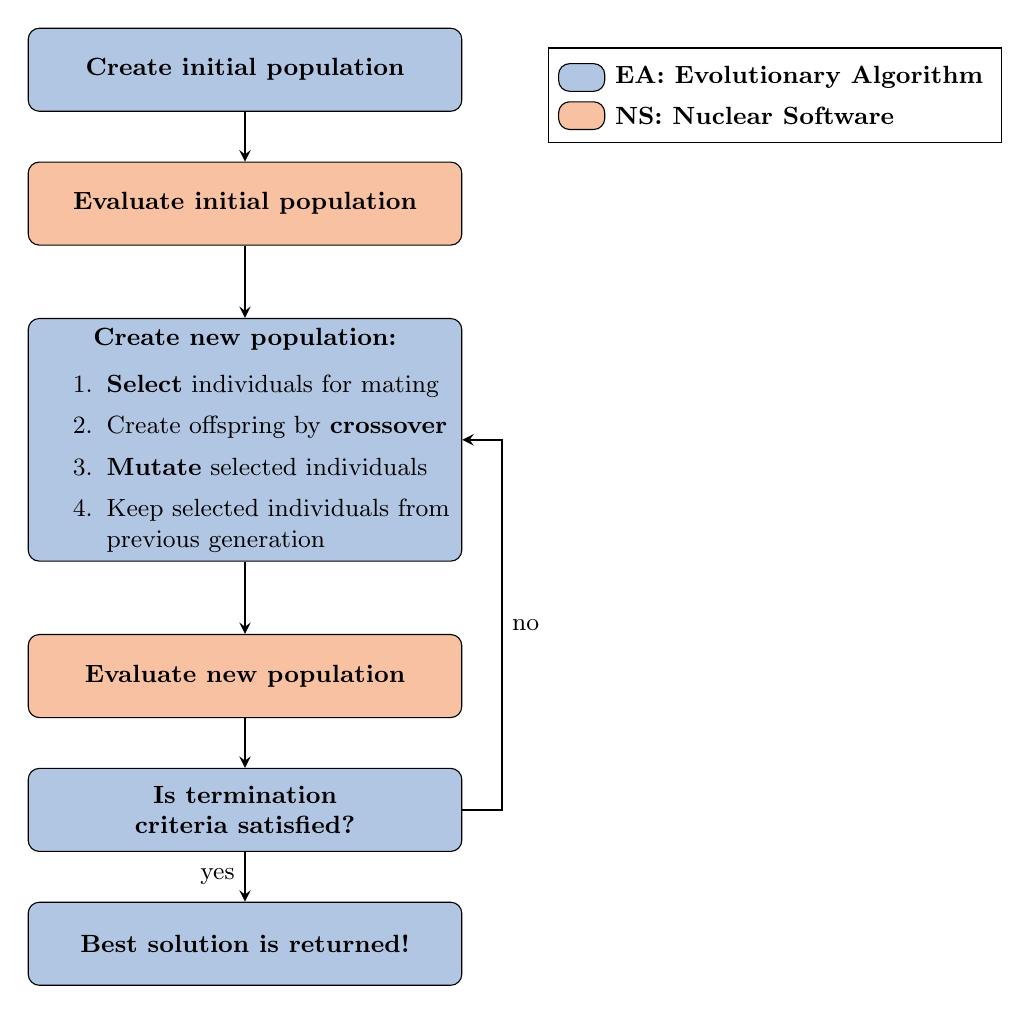
\begin{tikzpicture}[node distance=1.7cm]
            \tikzstyle{every node}=[font=\small]
            \node (1) [lbblock] {\textbf{Create initial population}};
            \node (2) [loblock, below of=1] {\textbf{Evaluate initial population}};
            \node (3) [lbblock, below of=2, yshift = -1.3cm] {\textbf{Create new population:} \\ 
            \begin{enumerate} \item \textbf{Select} individuals for mating 
                              \item Create offspring by \textbf{crossover} 
                              \item \textbf{Mutate} selected individuals 
                              \item Keep selected individuals from previous generation
                             \end{enumerate}};
            \node (4) [loblock, below of=3, yshift=-1.3cm] {\textbf{Evaluate new population}};
            \node (5) [lbblock, below of=4] {\textbf{Is termination \\ criteria satisfied?}};
            \node (6) [lbblock, below of=5] {\textbf{Best solution is returned!}};
            \draw [arrow] (1) -- (2);
            \draw [arrow] (2) -- (3);
            \draw [arrow] (3) -- (4);
            \draw [arrow] (4) -- (5);
            \draw [arrow] (5) -- node[anchor=east] {yes} (6);
            \draw [arrow] (5) -- ([shift={(0.5cm,0cm)}]5.east)-- node[anchor=west] {no} ([shift={(0.5cm,0cm)}]3.east)--(3);
            \matrix [draw,above right,yshift=10.7cm, xshift=0cm] at (current bounding box.south east) {
            \node [bbblock,label=right:\textbf{EA: Evolutionary Algorithm}] {}; \\
            \node [boblock,label=right:\textbf{NS: Nuclear Software}] {}; \\
            };
    \end{tikzpicture}
    \caption{Process of finding optimal solutions for a problem with a 
    genetic algorithm. Nuclear software evaluates each new population.}
    \label{fig:genetic_alg_nuclear}
\end{figure}
\gls{ROLLO} initially reads and validates the JSON input 
file, initializes the \gls{DEAP} \cite{fortin_deap_2012} genetic algorithm 
hyperparameters and operators, and finally runs the genetic algorithm following 
the flow chart in Figure \ref{fig:genetic_alg_nuclear}, in which the nuclear 
software evaluates each individual's fitness. 

% update this 
In the subsequent sections, I describe the evolutionary algorithm software (DEAP)
that drives \gls{ROLLO}, the nuclear software coupled to \gls{ROLLO}, and details about 
the \gls{ROLLO} framework, such as the input file format and software architecture. 

\section{Evolutionary Algorithm Driver}
Evolutionary algorithm computation uses sophisticated, diverse techniques 
and mechanisms, resulting in even the most well-designed, software frameworks 
being complicated under the hood. 
Utilizing an existing evolutionary algorithm framework presents implementation 
challenges as the user must edit the framework's source code to customize for their 
application and hyperparameters \cite{fortin_deap_2012}. 
Therefore, a computation framework that gives the user the capability to build 
custom evolutionary algorithms is ideal for this project.

Many evolutionary algorithm computation packages exist: 
\gls{DEAP} \cite{fortin_deap_2012}, inspyred \cite{garrett_inspyred_2014}, 
Pyevolve \cite{perone_pyevolve_2009}, and OpenBEAGLE \cite{gagne_open_2002}.
\gls{DEAP} is the newest package and places a high value on code 
compactness and clarity \cite{fortin_deap_2012}. 
\gls{DEAP} is the only framework that allows the user to prototype evolutionary 
algorithms rapidly and define custom algorithms without digging deep into 
the source code to modify hyperparameters and their application methods.
Accordingly, I chose \gls{DEAP} to drive the \gls{ROLLO} framework's 
evolutionary algorithm component. 
\gls{DEAP} provides building blocks for each optimizer function and allows the 
user to customize a specialized algorithm to fit their project \cite{fortin_deap_2012}.

\subsection{Distributed Evolutionary Algorithms in Python}
\gls{DEAP} is composed of two simples structures: a \textit{creator} and a 
\textit{toolbox}.  
The \textit{creator} module allows the run-time creation of classes via 
inheritance and composition, enabling individual and population creation from 
from any data structure: lists, sets, dictionaries, trees, etc \cite{fortin_deap_2012}. 
The \textit{toolbox} is a container that the user manually populates.
In the \textit{toolbox}, the user defines the selection, crossover, and 
mutation operator types and hyperparameters. 
For example, the user registers a crossover operator under the `mate'
alias, and a selection operator under the `select' alias. 
Then, the evolutionary algorithm uses these aliased operators from the 
\textit{toolbox}. 
If the user wants to change the crossover operator, they would update the 
`mate' alias in the \textit{toolbox}, while keeping the evolutionary algorithm 
unchanged \cite{fortin_deap_2012}. 

Figure \ref{fig:deap-code} illustrates \gls{DEAP}'s usage of the \textit{creator} and
\textit{toolbox} modules. 
\begin{figure}[]
    \begin{minted}[
        frame=lines,
        framesep=2mm,
        baselinestretch=1.2,
        fontsize=\footnotesize,
        linenos
        ]{python}
        
        from deap import creator, base, tools, algorithms
        creator.create("Objective", base.Fitness, weights=(-1.0,)) # minimum
        creator.create("Individual", list, fitness=creator.Objective)

        toolbox = base.Toolbox()
        toolbox.register("variable_1", random.uniform, 0.0, 10.0)
        toolbox.register("variable_2", random.uniform, -1.0, 0.0)
        def individual_creator():
            return creator.Individual([toolbox.variable_1(), toolbox.variable_2()])
        toolbox.register("individual", individual_creator())
        toolbox.register("population", tools.initRepeat, list, toolbox.individual)
        def evaluator_fn(individual):
            return tuple([sum(individual)])
        toolbox.register("evaluate", evaluator_fn)
        toolbox.register("select", tools.selBest, k=5)
        toolbox.register("mutate", tools.mutPolynomialBounded, eta=0.5, low=[0, -1], up=[-1, 0])
        toolbox.register("mate", tools.cxOnePoint)
    \end{minted}
    \caption{DEAP sample code demonstrating the usage of the \textit{creator} and
    \textit{toolbox} modules to initialize the genetic algorithm. In \gls{ROLLO}, \gls{DEAP}'s 
    \textit{creator} and \textit{toolbox} modules are initialized in the source 
    code based on the genetic algorithm parameters defined by the user in the 
    \gls{ROLLO} input file. }
    \label{fig:deap-code}
\end{figure}
Line 2 creates a single-objective fitness class, \texttt{Objective}. 
The first argument defines the name of the derived class, the second argument 
specifies the inherited base class, \texttt{base.fitness}, and the third 
argument indicates the objective fitness ($-1.0$ indicates a minimum objective, 
$+1.0$ indicates a maximum objective). 
Line 3 derives an \texttt{Individual} class from the standard Python list type,
and defines its fitness attribute to be the newly created \texttt{Objective} object. 
Lines 5-9 initialize the \gls{DEAP} toolbox, register 
\texttt{variable\_1} and \texttt{variable\_2} with their upper and lower bounds, 
and defines the \texttt{individual\_creator} function to return an 
\texttt{Individual} initialized with \texttt{variable\_1}, and \texttt{variable\_2}. 
Lines 10-11 and 14-17 are aliases for initializing individuals and population, 
specifying variation operators (\texttt{select}, \texttt{mutate}, \texttt{mate}), 
and evaluating individual fitness (\texttt{evaluate}) \cite{fortin_deap_2012}. 
Lines 12-13 define the evaluation function that returns the fitness values. 

\gls{ROLLO} initializes \gls{DEAP}'s \textit{creator} and \textit{toolbox} modules 
based on the genetic algorithm parameters defined by the user in the \gls{ROLLO} 
input file. 
The evaluation function runs the nuclear software and returns user-defined 
fitness values. 

\subsection{ROLLO Evolutionary Algorithm Implementation}
\gls{DEAP} creators provided variations of a classical genetic algorithm 
exposing different explicitness levels \cite{fortin_deap_2012}. 
The high-level examples use the built-in \gls{DEAP} genetic algorithms, 
whereas the low-level example completely unpacks the genetic algorithm to expose 
a generational loop. 

The general genetic algorithm included in ROLLO's \textbf{\textit{Algorithm}} class 
is an completely unpacked genetic algorithm. 
The algorithm begins by initializing the starting population and evaluating 
each individual's fitness value. 
Then, it enters a generational loop. 
During each iteration, the mating and mutation operators are applied to the population
to create an offspring population, and all offspring individuals are evaluated. 
The selection operator is then applied to both the old population 
and offspring population to select the best individuals to form 
the new population. 
Finally, the constraints are applied, and the results are saved.
Figure \label{fig:genetic_alg_nuclear} shows the algorithm's flow. 

Applying the selection operator to the combined old and offspring 
populations expands the population ensuring the effectiveness of 
elitism selection operators, such as NSGA-II, which work well 
for multi-objective optimization. 

\section{ROLLO Input File}
\gls{ROLLO}'s input file is in JSON format. 
There are four sections that the user must define: \\ \texttt{control\_variables}, 
\texttt{evaluators}, \texttt{constraints}, and \texttt{algorithm}. 
Figure \ref{fig:rollo-input} shows an example \gls{ROLLO} input file. 
In this simulation, \gls{ROLLO} uses a genetic algorithm with the defined 
hyperparameters to minimize the \texttt{output1} parameter which is 
calculated using the OpenMC evaluator that accepts input parameters: 
\texttt{variable1} and \texttt{variable2}. 
\begin{figure}[]
    \begin{minted}[
        frame=lines,
        framesep=2mm,
        baselinestretch=1.2,
        fontsize=\footnotesize,
        linenos
        ]{json}
        {
            "control_variables": {
                "variable1": {"min": 0.0, "max": 10.0}, 
                "variable2": {"min": -1.0, "max": 0.0}
            }, 
            "evaluators": {
                "openmc": {
                    "input_script": "openmc_inp.py",
                    "output_script": "openmc_output.py", 
                    "inputs": ["variable1", "variable2"],
                    "outputs": ["output1", "output2"]
                }
            }, 
            "constraints": {
                "output1": {"operator": [">=", "<"], "constrained_val": [1.0, 1.5]}
            }, 
            "algorithm": {
                "objective": ["min"], 
                "optimized_variable": ["output1"], 
                "pop_size": 100, 
                "generations": 10, 
                "mutation_probability": 0.23,
                "mating_probability": 0.46,
                "selection_operator": {"operator": "selTournament", "inds": 15, "tournsize":5},
                "mutation_operator": {
                    "operator": "mutPolynomialBounded",
                    "indpb": 0.23,
                    "eta": 0.23
                },
                "mating_operator": {"operator": "cxBlend", "alpha": 0.46}
            }
        }
    \end{minted}
    \caption{\acrfull{ROLLO} sample JSON input file.}
    \label{fig:rollo-input}
\end{figure}


\section{ROLLO Software Architecture}

\section{ROLLO Verification}

\section{ROLLO Stopping Criteria} %chapter 4
\chapter{AHTR Modeling and Optimization Methodology}
In this chapter, I describe the modeling and optimization methodology of
\gls{ROLLO} \gls{AHTR} optimization for non-conventional geometries and parameters.
To wholly explore the design space enabled by additive manufacturing, the 
optimization tool should enable placement of fuel, moderation, and coolant material 
in any possible location, within physical limits. 
Since exploration of non-conventional geometries and parameters has barely been
attempted (previous attempts described in Section \ref{sec:lit-review-reactor-arbitrary}), 
this dissertation attempts a first go at beginning to explore the large design space.  
The work done for this dissertation is only an intermediate step towards developing 
a truly arbitrary geometry expression. 

%In the subsequent sections, I will define the optimization problem, describe the 
%AHTR geometries . 
%Then, I will describe the software used to model them and the specific models. 

\section{Optimization Problem Definition}
\label{sec:opt-problem}
In an effort towards optimizing reactor design for non-conventional geometries 
and parameters.
I chose to vary the following \gls{AHTR} parameters: 
\begin{itemize}
    \item \gls{TRISO} particle packing fraction distribution, 
    $\rho_{TRISO}(\vec{r})$
    \item Total fuel packing fraction
    \item \gls{FLiBe} coolant channel shape 
\end{itemize} 
The TRISO packing fraction distribution variation enables exploration of how 
heterogenous fuel distributions impact reactor performance.
In Chapter \ref{chap:fhr-benchmark}, the results demonstrated that increased fuel 
packing does not always correspond with increased $k_{eff}$ due to self-shielding
effects. 
Varying total fuel packing fraction and TRISO distribution synergistically enables exploration of
how heterogenous TRISO distribution could minimize self-shielding and in turn reduce the fuel 
required for a reactor design. 
The FliBe coolant channel shape variation enables exploration of how non-uniform 
channel shapes impact reactor performance. 

I selected three key \gls{AHTR} optimization objectives that address contrasting reactor 
core qualities. 
Table \ref{tab:objectives} describes each objective, how I quantified them, and the motivation.
\begin{table}[]
    \centering
    \onehalfspacing
    \caption{\acrfull{ROLLO} optimization problem objectives with their quantification 
    descriptions, and motivation.}
	\label{tab:objectives}
    \footnotesize
    \begin{tabular}{p{4cm}p{5cm}p{5cm}}
    \hline 
    \textbf{Objective}& \textbf{Quantification}& \textbf{Motivation} \\
    \hline
    Minimize fuel amount & Minimize total fuel packing fraction & Cost savings, Non-proliferation \\ 
    \hline
    Maximize heat transfer & Minimize maximum temperature & Enable system to perform at a higher power with minimized thermal stress \\
    \hline
    Minimize power peaking & Minimize power peaking factor normalized by fuel distribution & Efficient fuel utilization, longer core life, safety\\
    \hline
    \end{tabular}
\end{table}
I will vary the described parameters in the \gls{AHTR} plank and \gls{AHTR} one-third assembly 
geometries to optimize the described objectives. 
The plank optimization acts as a preliminary study to inform the more complex \gls{AHTR} one-third
assembly optimization setup. 
In the next section, I will describe both geometries. 

\section{AHTR Geometry for Optimization Problem}
The optimization process is applied to both the \gls{AHTR} plank and \gls{AHTR} one-third
assembly geometries.
The geometries are adapted from the \gls{AHTR} design in the \gls{FHR} benchmark,
outlined in Chapter \ref{chap:fhr-benchmark}.
The main differences occur in the fuel plank region (see Figure \ref{fig:ahtr-fuel-assembly}). 
In the \gls{FHR} benchmark, the TRISO particles are arranged in rectangular lattices within
two fuel stripes in the plank. 
For the optimization problem, I instead discretized each plank into ten cells with random 
TRISO packing and an individually controlled packing fraction. 
I also omit the graphite spacers. 

\subsection{AHTR Plank Geometry}
\label{sec:ahtr-plank-geometry}
The \gls{AHTR} plank is a single graphite fuel plank model from the \gls{AHTR} design (Figure 
\ref{fig:ahtr-fuel-assembly}). 
I modified the fuel plank to be straightened with perpendicular sides, instead 
of slanted as in Figure \ref{fig:ahtr-fuel-plank}, for ease of modeling. 
The original slanted \gls{AHTR} geometry will be used for the complex one-third assembly 
optimization setup. 
Figure \ref{fig:straightened_plank} illustrates the straightened fuel plank with 
ten fuel cells with random \gls{TRISO} packing.
\begin{figure}[]
    \centering
    \includegraphics[width=0.85\linewidth]{straightened_plank.png}
    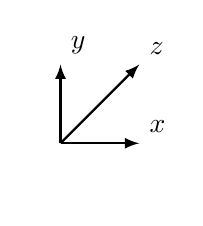
\begin{tikzpicture}
        \draw[ thick,-latex] (0,0) -- (1,0) node[anchor=south west] {$x$};
        \draw[ thick,-latex] (0,0) -- (0,1) node[anchor=south west] {$y$};
        \draw[ thick,-latex] (0,0) -- (1,1) node[anchor=south west] {$z$};
       \tkzText[above](-0.3,-0.7){}
       \end{tikzpicture} 
    \raggedright
    \resizebox{0.3\textwidth}{!}{
        \hspace{1cm}
        \fbox{\begin{tabular}{ll}
            \textcolor{fhrblue}{$\blacksquare$} & FLiBe \\
            \textcolor{fhrgrey}{$\blacksquare$} & Graphite (Structure)\\
            \textcolor{fhrred}{$\blacksquare$} & Graphite (Fuel Plank) \\
            \textcolor{fhrblack}{$\blacksquare$} & TRISO particle 

            \end{tabular}}}
    \caption{Straightened \acrfull{AHTR} fuel plank with 10 fuel cells with random 
    TRISO packing. Original slanted fuel planks can be seen in Figures 
    \ref{fig:ahtr-fuel-assembly} and \ref{fig:ahtr-fuel-plank}.}
    \label{fig:straightened_plank}
\end{figure}
The plank has $27.1 \times 3.25 \times 1.85\ cm^3$ dimensions with reflective 
boundary conditions.

I used the same materials as in the \gls{FHR} benchmark (Chapter \ref{chap:fhr-benchmark}), 
except that I homogenized each \gls{TRISO} particle's four outer layers: 
porous carbon buffer, inner pyrolytic carbon, silicon carbide layer, and the 
outer pyrolytic carbon. 
The \gls{TRISO} particle dimensions remain the same.
Table \ref{tab:keff_triso} reports OpenMC's reported $k_{eff}$ for this original 
straightened \gls{AHTR} configuration with and without the outer layer \gls{TRISO} 
homogenization.
\begin{table}[]
    \centering
    \onehalfspacing
    \caption{Straightened \acrfull{AHTR} fuel plank $k_{eff}$ for case with 
    no \gls{TRISO} homogenization and case with homogenization of the four outer 
    layers. Both simulations were run on one BlueWaters XE Node.}
	\label{tab:keff_triso}
    \footnotesize
    \begin{tabular}{llc}
    \hline 
    \textbf{TRISO Homogenization}& \textbf{$k_{eff}$} & \textbf{Simulation time [s]}  \\
    \hline 
    None & $1.38548 \pm 0.00124$ & 233\\ 
    Four outer layers & $1.38625 \pm 0.00109$ & 168\\ 
    \hline
    \end{tabular}
\end{table}
The \gls{TRISO} particle outer four-layer homogenization resulted in a $30\%$ 
speed-up without compromising accuracy with $k_{eff}$ values within each 
other's uncertainty.

% coolant channel shape variation

\subsection{AHTR One-Third Assembly Geometry}
The \gls{AHTR} one-third assembly is one-diamond shape sector of the \gls{AHTR} assembly and
contains six fuel planks.
Each graphite plank has graphite buffers and ten rectangular prism fuel cells 
with random TRISO packing and individually controlled packing fraction. 
Figure \ref{fig:ahtr_assembly} shows the one-third \gls{AHTR} assembly with 10 x 6 fuel cells with 
random \gls{TRISO} packing.
\begin{figure}[]
    \centering
    \begin{subfigure}{.7\textwidth}
    \includegraphics[width=\linewidth]{ahtr_assembly.png}
    \end{subfigure}%
    \begin{subfigure}{.3\textwidth}
        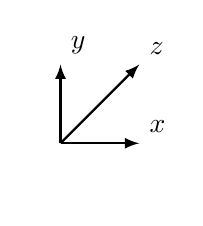
\begin{tikzpicture}
            \draw[ thick,-latex] (0,0) -- (1,0) node[anchor=south west] {$x$};
            \draw[ thick,-latex] (0,0) -- (0,1) node[anchor=south west] {$y$};
            \draw[ thick,-latex] (0,0) -- (1,1) node[anchor=south west] {$z$};
           \tkzText[above](-0.3,-0.7){}
        \end{tikzpicture} 
        \vspace{1cm}
        \fbox{\begin{tabular}{ll}
            \textcolor{fhrblue}{$\blacksquare$} & FLiBe \\
            \textcolor{fhrgrey}{$\blacksquare$} & Graphite (Structure)\\
            \textcolor{fhrred}{$\blacksquare$} & Graphite (Fuel Plank) \\
            \textcolor{fhrblack}{$\blacksquare$} & TRISO particle 
            \end{tabular}}
    \end{subfigure}
    \caption{\gls{AHTR} assembly with 10 fuel cells in each graphite plank with random 
    TRISO packing. Original \gls{FHR} benchmark fuel assembly with fuel stripes can be seen in 
    Figure \ref{fig:ahtr-fuel-assembly}.}
    \label{fig:ahtr_assembly}
\end{figure}
The assembly model also uses the \gls{TRISO} particle outer four layer homogenization described 
in Section \ref{sec:ahtr-plank-geometry}.

% coolant channel shape variation

\section{AHTR Model Workflow}
\gls{ROLLO} drives the evolutionary algorithm optimization process. 
In the \gls{ROLLO} input file, I will define control variables for the genetic algorithm 
to vary. 
These control variables are values used to control the \gls{AHTR} parameters described in 
Section \ref{sec:opt-problem}.
These control variables will be input into templated nuclear software to model different 
AHTR geometries.
The software will then run the \gls{AHTR} models and calculate the optimization objective 
and constraint values. 

In this work, I use OpenMC \cite{romano_openmc:_2015} to model \gls{AHTR}'s neutronics 
and Moltres \cite{lindsay_introduction_2018} to model the \gls{AHTR}'s multi-physics. 
OpenMC is an open-source Monte Carlo neutron transport code capable of 
performing k-eigenvalue calculations on models built using either constructive 
solid geometry or CAD representation. 
Moltres is an open-source tool designed to simulate \glspl{MSR} using 
deterministic neutronics and thermal-hydraulics implemented as an application 
atop the \gls{MOOSE} finite-element framework.  
Moltres solves arbitrary-group neutron diffusion, temperature, and precursor 
governing equations on a single mesh and can be deployed on an arbitrary number 
of processing units \cite{lindsay_introduction_2018}.
OpenMC and Moltres are both open-source, well-documented, well-supported, and 
Github version-controlled codes that can run in parallel on \gls{HPC} machines.

In this section, I describe the \gls{AHTR} modeling workflow: from the AHTR geometry 
variation input parameters, to the OpenMC and Moltres models, and finally the 
output and constraint values. 
This corresponds to the \textit{evaluate population} orange blocks in Figure 
\ref{fig:genetic_alg_nuclear}'s genetic algorithm flow chart.
Figure \ref{fig:ahtr-model-flow} illustrates the modeling workflow. 
\begin{figure}[]
    \centering
    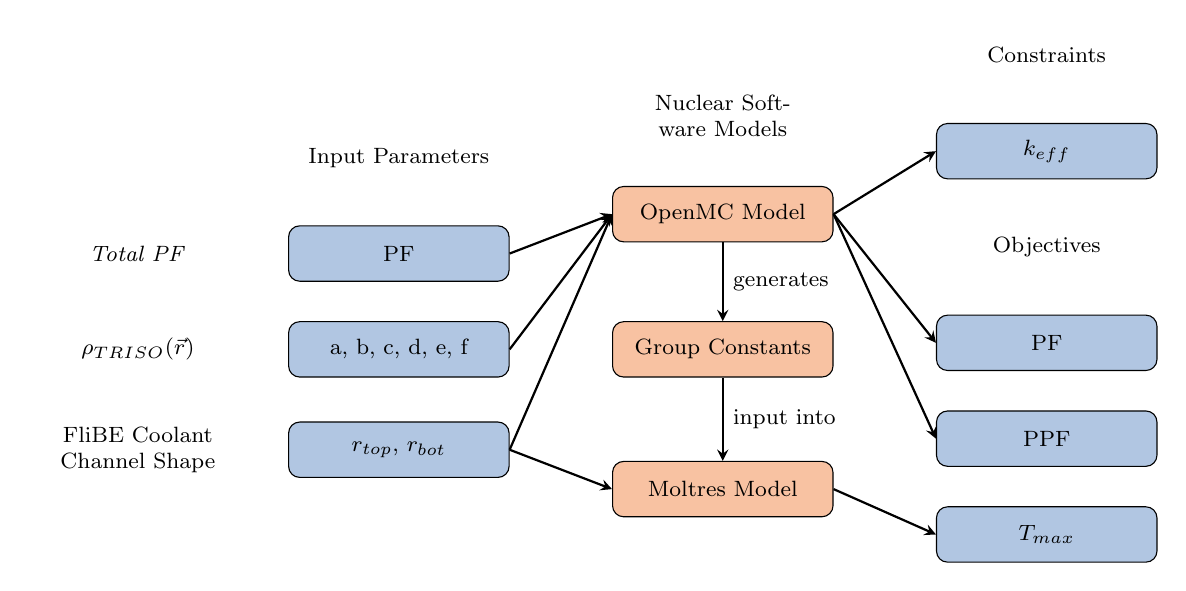
\begin{tikzpicture}[node distance=0.5cm]
        \tikzstyle{every node}=[font=\footnotesize]
        \node (1) [e72block] {\textit{Total PF}};
        \node (2) [b72block, right=of 1] {PF};
        \node (3) [e72block, above=of 2] {Input Parameters};
        \node (4) [e72block, below=of 1] {$\rho_{TRISO}(\vec{r})$};
        \node (5) [b72block, right=of 4] {a, b, c, d, e, f};
        \node (6) [e72block, below=of 4] {FliBE Coolant Channel Shape};
        \node (7) [b72block, right=of 6] {$r_{top}$, $r_{bot}$};
        \node (8) [o72block, right=of 2, xshift=0.8cm, yshift=0.5cm] {OpenMC Model};
        \node (9) [e72block, above=of 8] {Nuclear Software Models};
        \node (10) [o72block, right=of 5, xshift=0.8cm] {Group Constants};
        \node (11) [o72block, right=of 7, xshift=0.8cm, yshift=-0.5cm] {Moltres Model};
        \node (12) [b72block, right=of 8, xshift=0.8cm, yshift=0.8cm] {$k_{eff}$}; 
        \node (13) [e72block, above=of 12] {Constraints};
        \node (14) [e72block, below=of 12] {Objectives};
        \node (15) [b72block, below=of 14] {PF};
        \node (16) [b72block, below=of 15] {PPF};
        \node (17) [b72block, below=of 16] {$T_{max}$};
        \draw [arrow] (2) -- ([shift={(0cm,0cm)}]2.east) -- ([shift={(0cm,0cm)}]8.west);
        \draw [arrow] (5) -- ([shift={(0cm,0cm)}]5.east) -- ([shift={(0cm,0cm)}]8.west);
        \draw [arrow] (7) -- ([shift={(0cm,0cm)}]7.east) -- ([shift={(0cm,0cm)}]8.west);
        \draw [arrow] (7) -- ([shift={(0cm,0cm)}]7.east) -- ([shift={(0cm,0cm)}]11.west);
        \draw [arrow] (8) -- ([shift={(0cm,0cm)}]8.south) -- node[anchor=west] {generates} ([shift={(0cm,0cm)}]10.north);
        \draw [arrow] (10) -- ([shift={(0cm,0cm)}]10.south) -- node[anchor=west] {input into} ([shift={(0cm,0cm)}]11.north);
        \draw [arrow] (8) -- ([shift={(0cm,0cm)}]8.east) -- ([shift={(0cm,0cm)}]12.west);
        \draw [arrow] (8) -- ([shift={(0cm,0cm)}]8.east) -- ([shift={(0cm,0cm)}]15.west);
        \draw [arrow] (8) -- ([shift={(0cm,0cm)}]8.east) -- ([shift={(0cm,0cm)}]16.west);
        \draw [arrow] (11) -- ([shift={(0cm,0cm)}]11.east) -- ([shift={(0cm,0cm)}]17.west);
    \end{tikzpicture}
    \caption{\acrfull{AHTR} modeling workflow in ROLLO optimization.} 
    \label{fig:ahtr-model-flow}
\end{figure}

\subsection{Input Parameter Modeling}
In this section, I describe how I modeled the \gls{AHTR} parameter variations: total fuel packing 
fraction, \gls{TRISO} particle packing fraction distribution, and \gls{FLiBe} coolant channel shape. 
For both the \gls{AHTR} plank and one-third assembly models, total fuel packing fraction parameter 
is a single numerical input.
I describe the other two parameters for both the \gls{AHTR} plank and one-third assembly. 

\subsubsection{Input Parameter Modeling: TRISO particle packing fraction distribution}
For both the \gls{AHTR} plank and one-third assembly, I utilize sine distributions to govern the 
\gls{TRISO} particle packing fraction distribution. 
Based on the sine distributions, the model calculates the packing fraction in each fuel cell, then use 
OpenMC's \texttt{pack\_spheres} function to randomly disperse the calculated packing fraction in each 
fuel cell. 
For the \gls{AHTR} plank, one sine distribution governs the \gls{TRISO} packing fraction distribution 
across the fuel plank's x-direction. 
For the \gls{AHTR} one-third assembly, two sine distributions govern the \gls{TRISO} packing fraction 
distribution across each fuel plank's x-direction, and the assembly's y-direction, respectively. 

For the \gls{AHTR} plank, a sine distribution governs the \gls{TRISO} particle packing fraction 
distribution across the ten fuel cells, illustrated in Figure \ref{fig:straightened_plank}:
\begin{align}
    PF(x) &= \left(a\cdot sin(b\cdot x + c) + 2\right) \cdot NF\\
    \intertext{where}
    PF &= \mbox{packing fraction } [-] \nonumber \\ 
    a &= \mbox{amplitude, peak deviation of the function from zero } [-] \nonumber \\
    b &= \mbox{angular frequency, rate of change of the function argument } [\frac{radians}{cm}] \nonumber \\
    c &= \mbox{phase, the position in its cycle the oscillation is at t = 0 } [radians]\nonumber \\
    x &= \mbox{midpoint value for each cell } [cm]\nonumber \\
    NF &= \mbox{normalization factor } [-]\nonumber
\end{align}
The sine distribution's coefficients, \textit{a b c}, are the control variables \gls{ROLLO} 
utilizes to control the TRISO packing fraction distribution in the plank.
Thus, \gls{ROLLO} will vary $a, b, c$ constants to find an optimal TRISO particle 
sine distribution. 
The normalization factor ensures the correct total packing fraction 
in the plank regardless the \gls{TRISO} particle distribution.

For example in a \gls{AHTR} plank with a 0.0979 total packing fraction, and packing fraction 
distribution of $PF(x) = \left(0.5\cdot sin(\frac{\pi}{3}\cdot x + \pi) + 2\right)  \cdot NF$, 
results in the following packing fractions for the ten cells: 0.103, 0.120, 
0.049, 0.138, 0.076, 0.081, 0.136, 0.048, 0.125, and 0.098. 
Figure \ref{fig:triso_distribution} shows this sine distribution, highlights 
the packing fraction at the respective midpoints, and displays the plank's x-y 
axis view with packing fraction varying based on this sine distribution. 
\begin{figure}[]
    \centering
    \makebox[\textwidth][c]{\includegraphics[width=1.1\linewidth]{triso_distribution_sine.png}} 
    \caption{Above: Straightened \acrfull{AHTR} fuel plank with varying \gls{TRISO} particle 
    distribution across ten cells based on the sine distribution. 
    Below: $PF(x) = (0.5\ sin(\frac{\pi}{3}x + \pi) + 2)  \times NF$ 
    sine distribution with red points indicating the packing fraction at each cell. }
    \label{fig:triso_distribution}
\end{figure}

For the \gls{AHTR} one-third assembly, two sine distributions govern the x and y direction
\gls{TRISO} particle packing fraction distributions in the 10 x 6 fuel cell shape, illustrated in 
Figure \ref{fig:ahtr_assembly}:
\begin{align}
    PF(x, y) &= \left(a\cdot sin(b\cdot x + c) + 2\right) 
    \cdot \left(d\cdot sin(e\cdot y + f) + 2\right) \cdot NF \\
    \intertext{where}
    PF &= \mbox{packing fraction } [-] \nonumber \\ 
    a, d &= \mbox{amplitude, peak deviation of the function from zero } [-] \nonumber \\
    b, e &= \mbox{angular frequency, rate of change of the function argument } [\frac{radians}{cm}] \nonumber \\
    c, f &= \mbox{phase, the position in its cycle the oscillation is at t = 0 } [radians]\nonumber \\
    x &= \mbox{midpoint value for each x-direction fuel cell } [cm]\nonumber \\
    y &= \mbox{midpoint value for fuel plank } [cm]\nonumber \\
    NF &= \mbox{normalization factor } [-]\nonumber
\end{align}
The sine distribution's coefficients, \textit{a b c d e f}, are the control variables \gls{ROLLO} 
utilizes to control the TRISO packing fraction distribution in the assembly.
Thus, \gls{ROLLO} will vary \textit{a b c d e f} constants to find an optimal TRISO particle 
distribution. 
The normalization factor ensures the correct total packing fraction 
in the plank regardless the \gls{TRISO} particle distribution.

For example in an \gls{AHTR} one-third assembly with a 0.1 total packing fraction, and packing 
fraction distribution of $PF(x, y) = \left(0.5\cdot sin(1\cdot x + 1) + 2\right) \cdot 
\left(0.7\cdot sin(1.5\cdot y + 2) + 2\right) \cdot NF$ results in the packing fraction 
distribution shown in Figure \ref{fig:ahtr-assem-triso-distr-squares}.
This corresponds to the one-third assembly with varying TRISO distribution in its fuel 
cells, shown in Figure \ref{fig:ahtr-assem-triso-distr}. 
\begin{figure}[]
    \centering
    \begin{subfigure}{0.49\textwidth}
        \includegraphics[width=\linewidth]{ahtr-assem-triso-distr-squares.png}
        \caption{}
        \label{fig:ahtr-assem-triso-distr-squares} 
    \end{subfigure}
    \begin{subfigure}{0.49\textwidth}
        \includegraphics[width=\linewidth]{ahtr-assem-triso-distr.png}
        \raggedleft
        \resizebox{0.5\textwidth}{!}{
        \hspace{1cm}
        \fbox{\begin{tabular}{ll}
            \textcolor{fhrblue}{$\blacksquare$} & FLiBe \\
            \textcolor{fhrgrey}{$\blacksquare$} & Graphite (Structure) \\
            \textcolor{fhrred}{$\blacksquare$} & Graphite (Fuel Plank) \\
            \textcolor{fhrblack}{$\blacksquare$} & TRISO particle 
        \end{tabular}}}
        \caption{}
        \label{fig:ahtr-assem-triso-distr} 
    \end{subfigure}
    \caption{}
\end{figure}

\subsubsection{Input Parameter Modeling: FliBe Coolant Channel Shape}
I model the variation in coolant channel shape with a sinusoidal-like pattern.
I use cylinder surfaces in OpenMC, instead of a sinusoidal function. 
Creating complicated sinusoidal shapes in OpenMC requires the use of DAGMC, a CAD based tool, 
which is out of scope of the dissertation.
By varying the radius of the cylinder, the depth and frequency of the coolant channel shape 
minimics a sinusoidal-like pattern.
I vary the FliBE coolant channel shape while holding the total coolant area constant. 

For the \gls{AHTR} plank, $radius_{top}$ and $radius_{bot}$ variables control the coolant channel 
shape on the bottom and top FliBe channels. 
Figure \ref{fig:coolant-channel-shape} shows the \gls{AHTR} plank's coolant channel shape 
for $radius_{top} = 0.2$ and $radius_{bot} = 0.3$.
\begin{figure}[]
    \centering
        \includegraphics[width=\linewidth]{coolant-channel-shape.png}
    \raggedright
    \resizebox{0.3\textwidth}{!}{
        \hspace{1cm}
        \fbox{\begin{tabular}{ll}
            \textcolor{fhrblue}{$\blacksquare$} & FLiBe Coolant\\
            \textcolor{fhrgrey}{$\blacksquare$} & Graphite (Structure) \\
            \textcolor{fhrred}{$\blacksquare$} & Graphite (Fuel Plank) \\
            \textcolor{fhrblack}{$\blacksquare$} & TRISO particle 
        \end{tabular}}}
    \caption{AHTR Fuel Plank with Coolant Shape Variation, $radius_{top} 
    = 0.2$ and $radius_{bot} = 0.3$.}  
    \label{fig:coolant-channel-shape}
\end{figure}
$radius_{top}$ and $radius_{bot}$ are the control variables \gls{ROLLO} 
utilizes to control the coolant channel shape in the \gls{AHTR} plank.
Thus, \gls{ROLLO} will vary $radius_{top}$ and $radius_{bot}$ to find an optimal coolant 
channel shape.

% Assembly COolant channel shape variation

\subsection{AHTR OpenMC and Moltres Models}
\label{sec:ahtr-moltres-hom}
The input parameter modeling outlined in the previous section are inputs into 
the OpenMC neutronics model. 
The total packing fraction, TRISO particle distribution, and FliBE coolant 
channel shape are reflected in the OpenMC input file. 
Thus, there is TRISO level fidelity in the OpenMC neutronics model. 
The OpenMC neutronics model outputs the $k_{eff}$ constraint value, and the 
total packing fraction, and normalized power peaking factor output values. 
Section \ref{sec:ahtr_slab_output} gives further description of calculation for 
each output and constraint parameter.

For the Moltres model, a TRISO-level fidelity mesh file is impractical 
and will result in an extremely long Moltres runtimes. 
Moltres accepts group constant data from OpenMC for the Moltres multigroup 
neutron diffusion calculations and a mesh file representing the reactor geometry. 
Thus, for a successful \gls{AHTR} Moltres simulation, I established 
suitable spatial and energy homogenization that preserves accuracy while 
maintaining an acceptable runtime.
For both the \gls{AHTR} plank and one-third assembly models, I used the four group 
energy structure derived by Gentry et al. \cite{gentry_development_2016} for \gls{AHTR} 
geometries. 
Table \ref{tab:energy_structures} defines the group boundaries. 
\begin{table}[]
    \centering
    \onehalfspacing
    \caption{4-group energy structures for \acrfull{AHTR} geometry 
    derived by \cite{gentry_development_2016}.}
	\label{tab:energy_structures}
    \footnotesize
    \begin{tabular}{lll}
    \hline
    \multicolumn{3}{c}{\textbf{Group Boundaries [MeV]}} \\ 
    \hline
    \textbf{Group $\#$}& \textbf{Upper Bound} & \textbf{Lower Bound}  \\
    \hline 
    1 & $2.0000\times 10^1$ & $9.1188\times 10^{-3}$ \\ 
    2 & $9.1188\times 10^{-3}$ & $2.9023\times 10^{-5}$\\
    3 & $2.9023\times 10^{-5}$ & $1.8554\times 10^{-6}$\\
    4 & $1.8554\times 10^{-6}$ & $1.0000\times 10^{-12}$\\
    \hline
    \end{tabular}
\end{table}

For spatial homogenization of the straightened \gls{AHTR} fuel plank, I used 
OpenMC's \textit{cell} domain type to compute multigroup cross sections for 
different \textit{cells}. 
I discretized the plank into 13 \textit{cells}: FLiBe, left graphite, right 
graphite, and ten fuel cells (each cell has a different packing fraction). 
Figure \ref{fig:straightened_slab_mg} illustrates the \gls{AHTR} spatial 
homogenization for the OpenMC multigroup calculation. 
\begin{figure}[]
    \centering
    \includegraphics[width=\linewidth]{straightened_slab_mg.png}
    \raggedright
    \resizebox{0.5\textwidth}{!}{
        \hspace{1cm}
        \fbox{\begin{tabular}{llll}
            \textcolor{fhrblue}{$\blacksquare$} & FLiBe & 
            \textcolor{fhrgrey}{$\blacksquare$} & Left Graphite \\
            \textcolor{fhrred}{$\blacksquare$} & Right Graphite &
            \textcolor{fhrpink}{$\blacksquare$} & Fuel cell 1/6 \\
            \textcolor{fhryellow}{$\blacksquare$} & Fuel cell 2/7 &
            \textcolor{fhrorange}{$\blacksquare$} & Fuel cell 3/8 \\
            \textcolor{fhrgreen}{$\blacksquare$} & Fuel cell 4/9 &
            \textcolor{fhrpurple}{$\blacksquare$} & Fuel cell 5/10 \\
            \end{tabular}}}
    \caption{Straightened \acrfull{AHTR} fuel slab spatially discretized into 
    13 \textit{cells} for OpenMC multigroup calculation.}
    \label{fig:straightened_slab_mg}
\end{figure}

For spatial homogenization of the \gls{AHTR} one-third assembly... 
% include details about spatial homogenization for one-third assembly. 

To ensure that the spatial and energy homogenization preserves accuracy, I 
compared key neutronics parameters for the continuous OpenMC and multigroup 
Moltres simulations, for both the \gls{AHTR} plank and one-third assembly.
The results of the verification studies are described in Section 
\ref{sec:ahtr_model_verification}.

\subsection{Output Parameter Calculation}
\label{sec:ahtr_slab_output}
This section describes how I tallied the AHTR model outputs for the ROLLO 
optimization problem objectives (as described in Table \ref{tab:objectives}):
total fuel packing fraction, the maximum temperature in the slab, and 
normalized power peaking factor.  

\gls{ROLLO} will automatically return the total fuel packing fraction output parameter, 
since it is also an input parameter. 
In the Moltres AHTR model, I defined a post processor object to return the 
maximum temperature in the slab. 
To ensure efficient fuel utilization, one of the objectives is to minimize 
fuel-normalized power peaking in the slab, that takes into account fuel amount 
variations across the slab.
For the \gls{AHTR} plank, and each fuel plank in the \gls{AHTR} one-third fuel assembly I 
discretized the fuel cell area of the plank into 10 $\times$ 5 blocks.
I then use OpenMC to tally the fission energy production rate (\texttt{fission-q-recoverable}
$[eV/src]$) in each section.
I did not normalize the score to calculate power since the final PPF value is a 
ratio.
The normalized power peaking factor is calculated: 
\begin{align}
    PPF &= max(\frac{fqr_j}{PF_j}) \div ave(\frac{fqr_j}{PF_j})
\intertext{where}
j &= \mbox{discretized fuel area j} \nonumber \\
PPF &= \mbox{fuel-normalized power peaking factor} \nonumber \\
fqr_j &= \mbox{fission-q-recoverable at position j} \nonumber \\
PF_j &= \mbox{fuel packing fraction at position j} \nonumber
\end{align}

\section{AHTR Model Verification}
\label{sec:ahtr_model_verification}

\section{ROLLO Hyperparameter Tuning} % chapter 5
\chapter{AHTR Slab Optimization}
In this chapter, I demonstrated using \gls{ROLLO} to conduct \gls{AHTR} slab 
optimization for non-conventional geometries and parameters.
To wholly explore the design space enabled by additive manufacturing, the 
optimization tool should enable placement of fuel, moderation, and coolant material 
in any possible location, within physical limits. 
Since exploration of non-conventional geometries and parameters has not been done, 
a simple first attempt approach is taken for this dissertation. 

This chapter will explore optimizing the AHTR slab, while chapter 
\ref{ahtr_rollo_assembly} will explore optimizing the AHTR one-third fuel assembly.
In the subsequent sections, I describe the AHTR slab geometry, the optimization 
problem definition, AHTR slab modeling methods, and results of the 
single and multi objective \gls{AHTR} slab optimization problems.

\section{AHTR Slab Geometry}
% how the slab is set up etc
% 5.1.1 from prelim 
The \gls{AHTR} fuel slab used in this problem has straightened perpendicular 
sides, instead of slanted as in Figure \ref{fig:ahtr-fuel-plank}. 
Figure \ref{fig:straightened_slab} illustrates the straightened fuel slab.
\begin{figure}[H]
    \centering
    \includegraphics[width=0.85\linewidth]{straightened_slab.png}
    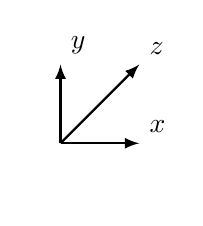
\begin{tikzpicture}
        \draw[ thick,-latex] (0,0) -- (1,0) node[anchor=south west] {$x$};
        \draw[ thick,-latex] (0,0) -- (0,1) node[anchor=south west] {$y$};
        \draw[ thick,-latex] (0,0) -- (1,1) node[anchor=south west] {$z$};
       \tkzText[above](-0.3,-0.7){}
       \end{tikzpicture} 
    \raggedright
    \resizebox{0.3\textwidth}{!}{
        \hspace{1cm}
        \fbox{\begin{tabular}{ll}
            \textcolor{fhrblue}{$\blacksquare$} & FLiBe \\
            \textcolor{fhrgrey}{$\blacksquare$} & Graphite (Fuel Plank)\\
            \textcolor{fhrred}{$\blacksquare$} & Graphite (Fuel Stripe) \\
            \textcolor{fhrblack}{$\blacksquare$} & TRISO particle 

            \end{tabular}}}
    \caption{Straightened \acrfull{AHTR} fuel slab with reflective boundary 
    conditions. Original slanted fuel slabs can be seen in Figures 
    \ref{fig:ahtr-fuel-assembly} and \ref{fig:ahtr-fuel-plank}.}
    \label{fig:straightened_slab}
\end{figure}
The slab has $27.1 \times 3.25 \times 1.85\ cm^3$ dimensions with reflective 
boundary conditions.
I use the same materials as in the \gls{FHR} benchmark (Chapter \ref{chap:fhr-benchmark}), 
except that I homogenized each \gls{TRISO} particle's four outer layers: 
porous carbon buffer, inner pyrolytic carbon, silicon carbide layer, and the 
outer pyrolytic carbon. 
The \gls{TRISO} particle dimensions remain the same.
Table \ref{tab:keff_triso} reports OpenMC's reported $k_{eff}$ for this original 
straightened \gls{AHTR} configuration with and without the outer layer \gls{TRISO} 
homogenization.
\begin{table}[H]
    \centering
    \onehalfspacing
    \caption{Straightened \acrfull{AHTR} fuel slab $k_{eff}$ for case with 
    no \gls{TRISO} homogenization and case with homogenization of the four outer 
    layers. Both simulations were run on one BlueWaters XE Node.}
	\label{tab:keff_triso}
    \footnotesize
    \begin{tabular}{llc}
    \hline 
    \textbf{TRISO Homogenization}& \textbf{$k_{eff}$} & \textbf{Simulation time [s]}  \\
    \hline 
    None & $1.38548 \pm 0.00124$ & 233\\ 
    Four outer layers & $1.38625 \pm 0.00109$ & 168\\ 
    \hline
    \end{tabular}
\end{table}
The \gls{TRISO} particle outer four-layer homogenization resulted in a $30\%$ 
speed-up without compromising accuracy with $k_{eff}$ values within each 
other's uncertainty.


\section{Optimization Problem Definition}
I limited the problem's scope to vary the following \gls{AHTR} parameters: 
\begin{itemize}
    \item \gls{TRISO} particle packing fraction distribution, $\rho_{TRISO}(\vec{r})$
    \item Total fuel packing fraction
    \item \gls{FLiBe} coolant channel shape 
\end{itemize} 
Three reactor optimization objectives were selected to address contrasting 
reactor core qualities. 
Table \ref{tab:objectives} describes the optimization objectives, how I quantified 
them, and the motivation for each.
\begin{table}[H]
    \centering
    \onehalfspacing
    \caption{\acrfull{ROLLO} optimization problem objectives with their quantification 
    descriptions, and motivation.}
	\label{tab:objectives}
    \footnotesize
    \begin{tabular}{p{4cm}p{5cm}p{5cm}}
    \hline 
    \textbf{Objective}& \textbf{Quantification}& \textbf{Motivation} \\
    \hline
    Minimize fuel amount & Minimize total fuel packing fraction & Cost savings, Non-proliferation \\ 
    \hline
    Maximize heat transfer & Minimize maximum temperature & Enable system to perform at a higher power with minimized thermal stress \\
    \hline
    Minimize power peaking & Minimize power peaking factor normalized by fuel distribution & Efficient fuel utilization, longer core life, safety\\
    \hline
    \end{tabular}
\end{table}
% top objectives of any reactor optimization process. 
% explain why each objective is important 
% should explore more optimization objectives, but this is good for 
% the scope of the dissertation
\gls{ROLLO} drives the evolutionary algorithm optimization process. 
\gls{ROLLO} varies the input parameters resulting in different AHTR slab geometries, 
the neutronics and multi-physics of the new geometries are then modeled in the 
OpenMC and Moltres software, these software calculate the problem's objective 
and constraint values. 
\gls{ROLLO} then iterates based on these results to find the 
input parameters that best optimize for the problem's objectives. 
Table \ref{tab:slab-obj-breakdown} shows the details of each \gls{ROLLO} 
optimization problem explored in this chapter.
\begin{table}[H]
    \centering
    \onehalfspacing
    \caption{\acrfull{ROLLO} simulations for optimizing \acrfull{AHTR}
    fuel slab. $PF$: Total Fuel Packing Fraction, $T_{max}$: Maximum Slab Temperature, 
    $PPF$: Normalized Power Peaking Factor, $\rho_{TRISO}(\vec{r})$: 
    \gls{TRISO} particle distribution}
	\label{tab:slab-obj-breakdown}
    \footnotesize
    \begin{tabular}{cllll}
    \hline 
    \textbf{Num Objectives} & \textbf{Objectives} & \textbf{Constraints} &\textbf{Varying Parameters} & \textbf{Simulation Software} \\
    \hline
    1 & \tabitem max($k_{eff}$) & - &\tabitem $\rho_{TRISO}(\vec{r})$ & OpenMC\\
    1 & \tabitem min($PF$) & \tabitem $k_{eff}$ $>$ 1.39 &\tabitem $\rho_{TRISO}(\vec{r})$ & OpenMC \\
      & & & \tabitem $PF$ & \\
    1 & \tabitem min($T_{max}$) & \tabitem $k_{eff}$ $>$ 1.0 &\tabitem $\rho_{TRISO}(\vec{r})$ & OpenMC, Moltres\\
    1 & \tabitem min($PPF$) & \tabitem $k_{eff}$ $>$ 1.0 &\tabitem $\rho_{TRISO}(\vec{r})$ & OpenMC\\
    1 & \tabitem min($PF$) & \tabitem $k_{eff}$ $>$ 1.39 &\tabitem FLiBe channel shape & OpenMC \\
      & & & \tabitem $PF$ & \\
    1 & \tabitem min($T_{max}$) & \tabitem $k_{eff}$ $>$ 1.0 &\tabitem FLiBe channel shape & OpenMC, Moltres\\
    1 & \tabitem min($PPF$) & \tabitem $k_{eff}$ $>$ 1.0 &\tabitem FLiBe channel shape & OpenMC\\
    \hline
    2 & \tabitem min($PF$) & $k_{eff}$ $>$ 1.39 & \tabitem $\rho_{TRISO}(\vec{r})$ & OpenMC, Moltres\\
      & \tabitem min($T_{max}$) & & \tabitem $PF$ & \\
    2 & \tabitem min($PF$) & $k_{eff}$ $>$ 1.39 & \tabitem $\rho_{TRISO}(\vec{r})$ & OpenMC\\
      & \tabitem min($PPF$) & & \tabitem $PF$ & \\
    2 & \tabitem min($T_{max}$) & $k_{eff}$ $>$ 1.0 & \tabitem $\rho_{TRISO}(\vec{r})$ & OpenMC, Moltres\\
      & \tabitem min($PPF$) & & & \\
    \hline
    3 & \tabitem min($PF$) & $k_{eff}$ $>$ 1.39 & \tabitem $\rho_{TRISO}(\vec{r})$ & OpenMC, Moltres\\
    & \tabitem min($PPF$) & & \tabitem $PF$ & \\
      & \tabitem min($T_{max}$) & & & \\
    \hline
    \end{tabular}
\end{table}

\section{AHTR Slab Modeling}
In this section, I describe the AHTR slab modeling workflow: from the AHTR geometry 
variation input parameters, to the OpenMC and Moltres models, and finally the 
output and constraint values. 
Figure \ref{fig:ahtr-slab-flow} illustrates the modeling workflow. 
\begin{figure}[H]
    \centering
    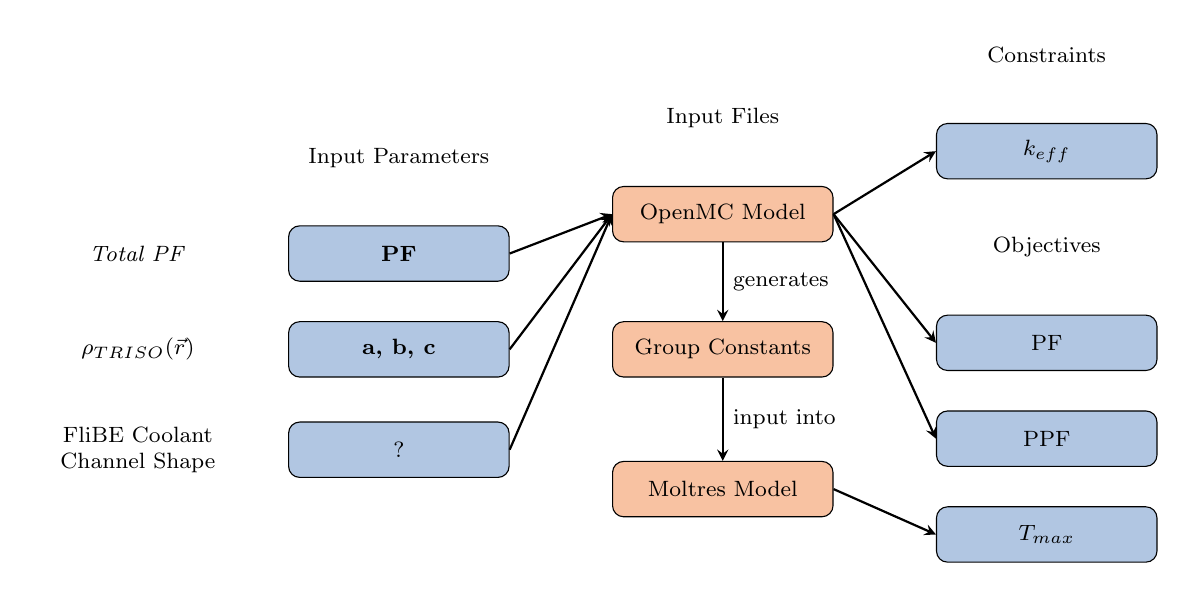
\begin{tikzpicture}[node distance=0.5cm]
        \tikzstyle{every node}=[font=\footnotesize]
        \node (1) [e72block] {\textit{Total PF}};
        \node (2) [b72block, right=of 1] {\textbf{PF}};
        \node (3) [e72block, above=of 2] {Input Parameters};
        \node (4) [e72block, below=of 1] {$\rho_{TRISO}(\vec{r})$};
        \node (5) [b72block, right=of 4] {\textbf{a, b, c}};
        \node (6) [e72block, below=of 4] {FliBE Coolant Channel Shape};
        \node (7) [b72block, right=of 6] {?};
        \node (8) [o72block, right=of 2, xshift=0.8cm, yshift=0.5cm] {OpenMC Model};
        \node (9) [e72block, above=of 8] {Input Files};
        \node (10) [o72block, right=of 5, xshift=0.8cm] {Group Constants};
        \node (11) [o72block, right=of 7, xshift=0.8cm, yshift=-0.5cm] {Moltres Model};
        \node (12) [b72block, right=of 8, xshift=0.8cm, yshift=0.8cm] {$k_{eff}$}; 
        \node (13) [e72block, above=of 12] {Constraints};
        \node (14) [e72block, below=of 12] {Objectives};
        \node (15) [b72block, below=of 14] {PF};
        \node (16) [b72block, below=of 15] {PPF};
        \node (17) [b72block, below=of 16] {$T_{max}$};
        \draw [arrow] (2) -- ([shift={(0cm,0cm)}]2.east) -- ([shift={(0cm,0cm)}]8.west);
        \draw [arrow] (5) -- ([shift={(0cm,0cm)}]5.east) -- ([shift={(0cm,0cm)}]8.west);
        \draw [arrow] (7) -- ([shift={(0cm,0cm)}]7.east) -- ([shift={(0cm,0cm)}]8.west);
        \draw [arrow] (8) -- ([shift={(0cm,0cm)}]8.south) -- node[anchor=west] {generates} ([shift={(0cm,0cm)}]10.north);
        \draw [arrow] (10) -- ([shift={(0cm,0cm)}]10.south) -- node[anchor=west] {input into} ([shift={(0cm,0cm)}]11.north);
        \draw [arrow] (8) -- ([shift={(0cm,0cm)}]8.east) -- ([shift={(0cm,0cm)}]12.west);
        \draw [arrow] (8) -- ([shift={(0cm,0cm)}]8.east) -- ([shift={(0cm,0cm)}]15.west);
        \draw [arrow] (8) -- ([shift={(0cm,0cm)}]8.east) -- ([shift={(0cm,0cm)}]16.west);
        \draw [arrow] (11) -- ([shift={(0cm,0cm)}]11.east) -- ([shift={(0cm,0cm)}]17.west);
    \end{tikzpicture}
    \caption{\acrfull{AHTR} fuel slab modeling workflow.} 
    \label{fig:ahtr-slab-flow}
\end{figure}

\subsection{Input Parameter Modeling}
In this section, I describe how I modeled the \gls{AHTR} input
parameter variations: total fuel packing fraction, TRISO particle packing fraction 
distribution, and \gls{FLiBe} coolant channel shape. 
The total fuel packing fraction is a single numerical input.

I vary the TRISO particle packing fraction across the fuel slab by dividing the 
slab into ten cells along the x-axis between the \gls{FLiBe} and graphite 
buffers, resulting in ten $2.31 \times 2.55 \times 1.85\ cm^3$ cells, and varying
the packing fraction in each cell.
A sine distribution governs the \gls{TRISO} particle packing fraction's 
distribution across cells:
\begin{align}
    PF(x) &= \left(a\cdot sin(b\cdot x + c) + 2\right) \cdot NF\\
    \intertext{where}
    PF &= \mbox{packing fraction } [-] \nonumber \\ 
    a &= \mbox{amplitude, peak deviation of the function from zero } [-] \nonumber \\
    b &= \mbox{angular frequency, rate of change of the function argument } [\frac{radians}{cm}] \nonumber \\
    c &= \mbox{phase, the position in its cycle the oscillation is at t = 0 } [radians]\nonumber \\
    x &= \mbox{midpoint value for each cell } [cm]\nonumber \\
    NF &= \mbox{Normalization factor } [-]\nonumber
\end{align}
The normalization factor ensures the correct total packing fraction 
in the slab regardless the \gls{TRISO} particle distribution.
I use OpenMC's \texttt{pack\_spheres} function to randomly disperse the calculated packing 
fraction in each fuel slab slice. 
For example, a total packing fraction of 0.0979, and packing fraction distribution of 
$PF(x) = \left(0.5\cdot sin(\frac{\pi}{3}\cdot x + \pi) + 2\right)  \cdot NF$, 
results in the following packing fractions for the ten cells: 0.103, 0.120, 
0.049, 0.138, 0.076, 0.081, 0.136, 0.048, 0.125, and 0.098. 
Figure \ref{fig:triso_distribution} shows this sine distribution, highlights 
the packing fraction at the respective midpoints, and displays the slab's x-y 
axis view with packing fraction varying based on this sine distribution. 
\begin{figure}[H]
    \centering
    \makebox[\textwidth][c]{\includegraphics[width=1.1\linewidth]{triso_distribution_sine.png}} 
    \caption{Above: Straightened \acrfull{AHTR} fuel slab with varying \gls{TRISO} particle 
    distribution across ten cells based on the sine distribution. 
    Below: $PF(x) = (0.5\ sin(\frac{\pi}{3}x + \pi) + 2)  \times NF$ 
    sine distribution with red points indicating the packing fraction at each cell. }
    \label{fig:triso_distribution}
\end{figure}
Thus, ROLLO will vary $a, b, c$ constants to find an optimal TRISO particle 
sine distribution. 

%% DESCRIPTION FOR COOLANT CHANNEL SHAPE DEFINITION.
I vary the FliBE coolant channel shape by: ...

\subsection{AHTR Slab OpenMC and Moltres Models}
\label{sec:ahtr-moltres-hom}
The input parameter modeling outlined in the previous section are inputs into 
the OpenMC neutronics model. 
The total packing fraction, TRISO particle distribution, and FliBE coolant 
channel shape are reflected in the OpenMC input file. 
Thus, there is TRISO level fidelity in the OpenMC neutronics model. 
The OpenMC neutronics model outputs the $k_{eff}$ constraint value, and the 
total packing fraction, and normalized power peaking factor output values. 
Section \ref{sec:ahtr_slab_output} gives further description of calculation for 
each output and constraint parameter.

For the Moltres model, a TRISO-level fidelity mesh file is impractical 
and will result in an extremely long Moltres runtimes. 
Moltres accepts group constant data from OpenMC for the Moltres multigroup 
neutron diffusion calculations and a mesh file representing the reactor geometry. 
Thus, for a successful \gls{AHTR} Moltres simulation, I established 
suitable spatial and energy homogenization that preserves accuracy while 
maintaining an acceptable runtime.

For spatial homogenization of the straightened \gls{AHTR} fuel slab, I used 
OpenMC's \textit{cell} domain type to compute multigroup cross sections for 
different \textit{cells}. 
I discretized the slab into 13 \textit{cells}: FLiBe, left graphite, right 
graphite, and ten fuel cells (each cell has a different packing fraction). 
Figure \ref{fig:straightened_slab_mg} illustrates the \gls{AHTR} spatial 
homogenization for the OpenMC multigroup calculation. 
\begin{figure}[H]
    \centering
    \includegraphics[width=\linewidth]{straightened_slab_mg.png}
    \raggedright
    \resizebox{0.5\textwidth}{!}{
        \hspace{1cm}
        \fbox{\begin{tabular}{llll}
            \textcolor{fhrblue}{$\blacksquare$} & FLiBe & 
            \textcolor{fhrgrey}{$\blacksquare$} & Left Graphite \\
            \textcolor{fhrred}{$\blacksquare$} & Right Graphite &
            \textcolor{fhrpink}{$\blacksquare$} & Fuel cell 1/6 \\
            \textcolor{fhryellow}{$\blacksquare$} & Fuel cell 2/7 &
            \textcolor{fhrorange}{$\blacksquare$} & Fuel cell 3/8 \\
            \textcolor{fhrgreen}{$\blacksquare$} & Fuel cell 4/9 &
            \textcolor{fhrpurple}{$\blacksquare$} & Fuel cell 5/10 \\
            \end{tabular}}}
    \caption{Straightened \acrfull{AHTR} fuel slab spatially discretized into 
    13 \textit{cells} for OpenMC multigroup calculation.}
    \label{fig:straightened_slab_mg}
\end{figure}
I used the four group energy structure derived by Gentry et al. 
\cite{gentry_development_2016} for \gls{AHTR} geometries. 
Table \ref{tab:energy_structures} defines the group boundaries. 
\begin{table}[H]
    \centering
    \onehalfspacing
    \caption{4-group energy structures for \acrfull{AHTR} geometry 
    derived by \cite{gentry_development_2016}.}
	\label{tab:energy_structures}
    \footnotesize
    \begin{tabular}{lll}
    \hline
    \multicolumn{3}{c}{\textbf{Group Boundaries [MeV]}} \\ 
    \hline
    \textbf{Group $\#$}& \textbf{Upper Bound} & \textbf{Lower Bound}  \\
    \hline 
    1 & $2.0000\times 10^1$ & $9.1188\times 10^{-3}$ \\ 
    2 & $9.1188\times 10^{-3}$ & $2.9023\times 10^{-5}$\\
    3 & $2.9023\times 10^{-5}$ & $1.8554\times 10^{-6}$\\
    4 & $1.8554\times 10^{-6}$ & $1.0000\times 10^{-12}$\\
    \hline
    \end{tabular}
\end{table}

To ensure that the spatial and energy homogenization preserves accuracy, I 
compared key neutronics parameters for the continuous OpenMC and multigroup 
Moltres simulations.

\subsection{Moltres Model Neutronics Performance Verification}
In this section, I set up a criticality eigenvalue problem in Moltres to demonstrate  
it's ability to reproduce key neutronics parameters using multi-group constant 
data from OpenMC for the AHTR slab.  
The accuracy from this neutronics verification step gives confidence for 
subsequent AHTR slab multiphysics simulations with Moltres. 

% move this to lit review for Moltres
Moltres solves the four-group diffusion equations as a steady-state eigenvalue 
problem to find $k_{eff}$ for the static AHTR slab model: 
\begin{align}
    \frac{1}{v_g} \frac{\partial \phi_g}{\partial t} &= \nabla \cdot D_g
    \nabla \phi_g - \Sigma^r_g \phi_g +
    \sum^G_{g' \neq g} \Sigma^s_{g' \rightarrow g} \phi_{g'} + \chi^p_g
    \sum^G_{g'=1} (1-\beta) \nu \Sigma^f_{g'} \phi_{g'} + \chi^d_g \sum^I_i
    \lambda_i C_i
\end{align}

I will be comparing the key neutronics parameters between two simulations:
\begin{enumerate}
    \item OpenMC simulation with continuous energy and TRISO-level spatial fidelity 
    \item Moltres simulation with 4-group energy and 13-cell spatial homogenization
\end{enumerate}
I outlined the spatially homogenization used in section ??. 
The OpenMC simulation with TRISO-level fidelity generates the group 
constants for the energy and spatially homogenized Moltres simulation. 

% Describe how you calculated each simulation. MGXS generation and group 
% constant generation

% say i changed it to reflective and temperature = 948K

\subsubsection{Effective Multiplication Factor}
In this section, I include results from a homogenized OpenMC simulation as well to 
distinguish between differences caused by spatial homogenization, and differing 
OpenMC and Moltres normalization and solving methods. 
% explain how this works 
\begin{table}[H]
    \centering
    \onehalfspacing
    \caption{AHTR Fuel Slab's $k_{eff}$ values from OpenMC and Moltres at 948K.
    Normalized difference is the pcm difference normalized by $k_{eff}$}
	\label{tab:keff_ahtr_moltres}
    \footnotesize
    \begin{tabular}{lllcc}
    \hline 
    \textbf{Software}& \textbf{Homogenized?}& \textbf{$k_{eff}$} & \textbf{Difference [pcm]}  
    & \textbf{Normalized Difference [pcm]}\\
    \hline 
    OpenMC & No & $1.41402 \pm 0.00140$ & - & -\\ 
    OpenMC & Yes & $1.41473 \pm 0.00098$ & +71 & -\\ 
    Moltres & Yes & $1.40696 $ & -706 & -502\\ 
    \hline
    \end{tabular}
\end{table}
The 71pcm $k_{eff}$ difference between continuous and homogenized OpenMC 
simulations show that the selected spatial and energy homogenizations
are acceptable. 
However, there is a 502pcm difference in the Moltres simulation's $k_{eff}$.
Possible reasons are that the neutron diffusion method used in Moltres does not 
approximate this reactor geometry as well. 
The diffusion coefficients for this reactor type are approximately 1cm. 
The FliBE coolant channel has a 0.35cm width which is smaller than the diffusion
coefficient, resulting in poor approximations. 

\subsubsection{Reactivity Coefficients}
Moltres' delayed neutron fraction, $\beta{eff}$, is calculated by taking the 
normalized difference between $k_{eff}$ values with and without DNPs. 
The  $\beta{eff}$ values from OpenMC and Moltres show excellent 
agreement with a discrepancy of 0.1pcm. 
\begin{table}[H]
    \centering
    \onehalfspacing
    \caption{AHTR Fuel Slab's $\beta_{eff}$ values from OpenMC and Moltres at 948K.}
	\label{tab:betaeff_ahtr_moltres}
    \footnotesize
    \begin{tabular}{lllc}
    \hline 
    \textbf{Software}& \textbf{Homogenized?}& \textbf{$\beta_{eff}$ [pcm]} 
    & \textbf{Difference [pcm]}  \\
    \hline 
    OpenMC & No &  654.3 & - \\ 
    Moltres & Yes & 654.4 & 0.1\\ 
    \hline
    \end{tabular}
\end{table}
I calculated the temperature reactivity coefficients with equation ??. % FHR BM section
Temperature reactivity feedback arises mainly from Doppler broadening of 
resonance absorption peaks and thermal expansion.
The total temperature coefficients from OpenMC and Moltres show good 
agreement with a discrepancy of 0.4 pcm/K.
\begin{table}[H]
    \centering
    \onehalfspacing
    \caption{AHTR Fuel Slab's total reactivity coefficient values calculated from 
    OpenMC and Moltres at 948K and 1100K.}
	\label{tab:reactivity_ahtr_moltres}
    \footnotesize
    \begin{tabular}{lllc}
    \hline 
    \textbf{Software}& \textbf{Homogenized?}& \textbf{Total $\frac{\Delta \rho}{\Delta T}$ [pcm/K]} 
    & \textbf{Difference [pcm/K]}  \\
    \hline 
    OpenMC & No &  -8.4 & - \\ 
    Moltres & Yes & -8.8 & -0.4\\ 
    \hline
    \end{tabular}
\end{table}

\subsubsection{Flux Distribution}
Moltres' source term ($Q_f$) is defined by: 
\begin{align}
\label{eq:moltres-source-term}
    Q_f &= \sum_{g=1}^G \epsilon_{f,g}\Sigma_{f,g}\phi_g
\intertext{where} 
Q_f &= \mbox{source term } [\frac{MeV}{cm^3s}] \nonumber \\
G &= \mbox{number of discrete groups, g } [-] \nonumber \\
\epsilon_{f,g} &= \mbox{heat produced per fission } [MeV] \nonumber \\
\Sigma_{f,g} &= \mbox{macroscopic cross section for fission due to neutrons in group g } [\frac{1}{cm}] \nonumber \\
\phi_g &= \mbox{flux of neutrons in group g } [\frac{n}{cm^2s}]\nonumber
\end{align}
The $\epsilon_{f,g}$ and $\Sigma_{f,g}$ terms are provided to Moltres through 
the group constants generated by neutronics software, OpenMC.
Thus, differences in the source term between OpenMC and Moltres are dependent on 
the flux. 
Comparison of flux distributions produced by Moltres and OpenMC are key to 
ensuring that temperature distribution is accurately calculated in Moltres.

Figure \ref{fig:flux_948K} shows the 4-group flux distributions for OpenMC and 
Moltres. 
\begin{figure}[H]
    \centering
    \includegraphics[width=0.48\linewidth]{flux_group1_948K.png} 
    \includegraphics[width=0.48\linewidth]{flux_group2_948K.png} 
    \includegraphics[width=0.48\linewidth]{flux_group3_948K.png} 
    \includegraphics[width=0.48\linewidth]{flux_group4_948K.png} 
    \caption{AHTR fuel slab's centerline neutron flux distribution in 4 groups
    at 948K. 
    Energy Group 1: E $> 9.1188 \times 10^{-3}$ MeV, 
    Energy Group 2: $2.9023 \times 10^{-5} < E < 9.1188 \times 10^{-3}$ MeV,
    Energy Group 3:  $1.8556 \times 10^{-5} < E < 2.9023 \times 10^{-5}$ MeV,
    Energy Group 4:  $1.0 \times 10^{-12} < E < 1.8554 \times 10^{-6}$ MeV}
    \label{fig:flux_948K}
\end{figure}
The OpenMC simulation shows higher flux in Group 1, and lower flux in the
Group 2 and Group 3. 
However, there is an overall good agreement for each group's flux.  

\subsubsection{Neutron Energy Spectrum}
Figure \ref{fig:neutron_spectrum_948K} shows the neutron spectrum the OpenMC simulation 
for both 252 and 4 , and 4-group Moltres simulation. 

 \begin{figure}[H]
    \centering
    \includegraphics[width=\linewidth]{neutron_spectrum_948K.png}
    \caption{AHTR fuel slab's neutron spectrum.}  
    \label{fig:neutron_spectrum_948K}
\end{figure}

In summary, Moltres replicated the relevant neutronics parameters accurately 
using group constant data from OpenMC. % more description

\subsection{Moltres AHTR Steady-State Temperature Model}
\label{sec:ahtr-moltres-model}
% how to model heat transfer for constant coolant channel shape and varying shape 
One of the ROLLO AHTR optimization objectives is minimizing the maximum 
temperature in the slab. 
A neutronics simulation cannot calculate maximum temperature; thus, I introduced 
AHTR slab temperature modeling with Moltres.
In the next sections, I discuss group constant generation and describe the Moltres 
temperature model. 

\subsubsection{Group Constant Generation}
I used OpenMC to generate multigroup neutronics data for the AHTR slab 
for four energy groups and eight precursor groups based on the spatial and 
energy homogenization described in section \ref{sec:ahtr-moltres-hom}.
Moltres has the capability 
% multiple temperatures in group constants, interpolation 

\subsubsection{Temperature Model}
The Moltres AHTR Steady-State Temperature Model first solves for the neutronics 
in slab and uses that to solve for the temperature distribution in the slab 
for a defined power. 
The temperature model assumes conductive heat transfer throughout the domain 
and heat removal by uniform salt flow in the coolant region. 
These assumptions ignore flow and turbulent effects that would most likely be 
present. 
However, an in-depth AHTR Moltres model that includes turbulence model is 
out of scope for this dissertation. 

Equation \ref{eq:moltres-temp} described Moltres' governing equation for 
temperature.
In the 2D cross-sectional AHTR Steady-State Temperature Model, I ignore the 
time-dependent and velocity-dependent terms since I am solving for steady-state 
and there is no moving fuel: 
\begin{align}
    - \nabla \cdot (k_i \nabla T) &= Q_i
\intertext{where:}
k_i &= \mbox{thermal conductivity of material i} \nonumber \\
T &= \mbox{temperature in the slab} \nonumber \\
Q_i &= \mbox{source or sink term in material i} \nonumber
\end{align} 
I use insulated temperature boundary conditions.  
Table \ref{tab:ahtr-thermal-conducitivity} shows the thermal conductivity values 
used for each AHTR slab material. 
\begin{table}[H]
    \centering
    \onehalfspacing
    \caption{AHTR Fuel Slab materials' thermal conductivity.}
	\label{tab:ahtr-thermal-conducitivity}
    \footnotesize
    \begin{tabular}{lp{4cm}l}
    \hline 
    \textbf{Material}& \textbf{Thermal Conductivity [$Wcm^{-1}K^{-1}$]}& \textbf{References} \\ 
    \hline 
    FliBE & 0.01 & \\
    Graphite  & 0.15 & \\
    Fuel  & 0.099 & \\
    \hline
    \end{tabular}
\end{table}
Equation \ref{eq:moltres-source-term} defines the fuel cells' fission source term.
Equation \ref{eq:moltres-heat-removal} defines the heat removal from the AHTR 
fuel slab in the coolant areas: 
\begin{align}
    \label{eq:moltres-heat-removal}
    Q &= h \cdot (T(\vec{r})-T_{ref})
\intertext{where:}
Q &= \mbox{heat removal rate for 1cm thin slice of AHTR slab [W/cm]} \nonumber \\
h &= \mbox{heat transfer coefficient } [\frac{W}{cm \cdot K}] \nonumber \\
T(\vec{r}) &= \mbox{temperature at point $\vec{r}$ [K]} \nonumber \\
T_{ref} &= \mbox{reference temperature [K]} \nonumber
\end{align}

Table \ref{tab:heat-exchanger-constants} shows the values used for 
reference temperature and heat transfer coefficient for the convective 
heat transfer process.
\begin{table}[H]
    \centering
    \onehalfspacing
    \caption{AHTR Fuel Slab's heat transfer constants.}
	\label{tab:heat-exchanger-constants}
    \footnotesize
    \begin{tabular}{llll}
    \hline 
    \textbf{Constant}& \textbf{Value}& \textbf{Units} & \textbf{Notes} \\
    \hline 
    h & 990 & $\frac{W}{cm \cdot K}$ & Calculated in Eq. \ref{eq:calc-htc} \\
    $T_{ref}$ & 923 & K & AHTR Inlet Temperature \\ %cite ahtr 923K inlet temp 
    \hline
    \end{tabular}
\end{table} 
I calculated the heat transfer coefficient ($h$) using Equation \ref{eq:calc-htc} 
for the 1cm-thick AHTR $\Delta z$ slice with the following assumptions: 
\begin{itemize}
    \item it generates a constant amount of power, all of which is removed 
    by the coolant
    \item heat removal occurs at the coolant areas
    \item temperature increase per 1cm slice is constant from the inlet to the 
    outlet 
\end{itemize} 
\begin{align}
    \label{eq:calc-htc}
    h &= \frac{P_{dz}}{A_{coolant}} \div \frac{T_{total}}{H} \\
      &= \frac{1456 W}{23.1 * 0.5 * 2 cm^2} / (50 K / 550 cm) \nonumber \\
      &= 990 W cm^{-1}K^{-1} \nonumber 
\intertext{where:}
h &= \mbox{heat transfer coefficient } [\frac{W}{cm \cdot K}] \nonumber \\
P_{dz} &= \mbox{power produced in 1cm AHTR slab dz slice [$W$]}\nonumber \\
A_{coolant} &= \mbox{cross-sectional coolant area in AHTR slab [$cm^2$]} \nonumber \\
T_{total} &= \mbox{total temperature change from inlet to outlet [$K$]} \nonumber \\
H &= \mbox{AHTR height from inlet to outlet [$cm$]} \nonumber 
\end{align}
In the ROLLO optimization simulations, I vary the FliBE coolant channel shape. 
During the shape variation, I hold the coolant area constant. 
Therefore, the Moltres temperature model holds the heat transfer coefficient ($h$)
constant for all the simulations.  

Using the described models and assumptions, I set up a Moltres AHTR steady-state 
temperature model for a slab with a constant packing fraction of 0.0979 across ten 
fuel cells. 
The \texttt{constant$\_$0.0979} directory in the \texttt{2022-chee-dissertation} 
Github repository contains the model. % cite DOI   
Figure \ref{fig:ahtr_constant_temp} shows the Moltres-generated temperature 
distribution with an average and maximum temperature of 1019K and 1128K, 
respectively.
\begin{figure}[H]
    \centering
    \includegraphics[width=\linewidth]{ahtr_constant_temp.png}
    \caption{AHTR fuel slab's Moltres generated temperature distribution for a 
    slab with a constant packing fraction of 0.0979 across ten fuel cells.}  
    \label{fig:ahtr_constant_temp}
\end{figure}
The temperature distribution is consistent with previous temperature models of 
the AHTR fuel slabs that report an average fuel kernel temperature of 1125K 
\cite{ramey_methodology_2021}. 
Model differences include that Ramey \cite{ramey_methodology_2021} utilized a 
1D temperature model with the original 4-layer TRISO model from the FHR benchmark 
(Figure \ref{fig:straightened_slab}).
This model is 2D and randomly disperses TRISO particles throughout the 
slab while keeping the same overall packing fraction. 
Chapter \ref{chap:fhr-multiphysics-model} conducts a more accurate one-for-one 
comparison \ref{chap:fhr-multiphysics-model}.

% Discuss convergence of Moltres temperature model 

\subsection{Output Parameter Calculation}
\label{sec:ahtr_slab_output}
% PF, Max temp, PPF 
This section describes how I tallied the AHTR model outputs for the ROLLO 
optimization problem objectives (as described in Table \ref{tab:objectives}):
total fuel packing fraction, the maximum temperature in the slab, and 
normalized power peaking factor.  

ROLLO will automatically return the total fuel packing fraction output parameter, 
since it is also an input parameter. 
In the Moltres AHTR slab model, I defined a post processor object to return the 
maximum temperature in the slab. 

To ensure efficient fuel utilization, one of the objectives is to minimize 
fuel-normalized power peaking in the slab, that takes into account fuel amount 
variations across the slab.
I discretized the fuel cell area of the slab into 10 $\times$ 5 blocks, and 
use OpenMC to tally the fission energy production rate (\texttt{fission-q-recoverable}
$[eV/src]$) in each section.
I did not normalize the score to calculate power since the final PPF value is a 
ratio.
% why fission q recoverable
The normalized power peaking factor is calculated: 
\begin{align}
    PPF &= max(\frac{fqr_j}{PF_j}) \div ave(\frac{fqr_j}{PF_j})
\intertext{where}
j &= \mbox{discretized fuel area j} \nonumber \\
PPF &= \mbox{fuel-normalized power peaking factor} \nonumber \\
fqr_j &= \mbox{fission-q-recoverable at position j} \nonumber \\
PF_j &= \mbox{fuel packing fraction at position j} \nonumber
\end{align}

\section{Optimization Results}
In this section, I report the results from the ROLLO optimization simulations 
outlined in Table \ref{tab:slab-obj-breakdown}.
Results from this section can be found in the \texttt{2022-chee-dissertation} 
Github repository under the \texttt{rollo-ahtr-slab} directory. %cite 

\subsection{Single-Objective Optimization}
In this section, I report the results for single objective optimization. 

\subsubsection{Objective: Minimize Total Packing Fraction}
I varied the TRISO particle distribution and total packing fraction, while
constraining $k_{eff} >= 1.39$. % why 1.39
Figure \ref{fig:slab-obj-1-pf-evol} shows the total packing fraction evolution and 
figure \ref{fig:slab-obj-1-pf-final} shows the five TRISO particle distributions in 
the final generation with the smallest packing fraction. 
\begin{figure}[]
    \centering
    \begin{subfigure}{\textwidth}
        \includegraphics[width=\linewidth]{slab-obj-1-pf-evol.png}
        \caption{Minimum, average, and maximum total packing fraction evolution.}
        \label{fig:slab-obj-1-pf-evol} 
    \end{subfigure}
    \begin{subfigure}{\textwidth}
        \includegraphics[width=\linewidth]{slab-obj-1-pf-final.png}
        \caption{TRISO particle distribution for the 5 individuals with the 
        smallest packing fraction in generation 9.}
        \label{fig:slab-obj-1-pf-final} 
    \end{subfigure}
    \caption{ROLLO single-objective optimization to minimize total packing fraction. 
    Input parameters varied: total packing fraction, TRISO particle distribution.}
    \label{fig:slab-obj-1-pf}
\end{figure}
The minimum and average packing fractions converged very quickly, as expected 
in this single-objective optimization problem.
By the $9^{th}$ generation, the average, minimum, and maximum packing fraction
values converged to approximately 0.023. 
In figure \ref{fig:slab-obj-1-pf-final}, I observe that the TRISO particle packing 
sine distributions are not exactly the same, but follow a similar pattern of 
alternating between a higher packing fraction, and a lower packing fraction 
in the neighboring fuel cell. 
The up-down fuel packing pattern minimizes self-shielding effects, enabling  
a lower packing fraction for the same $k_{eff}$. 

\subsubsection{Objective: Minimize Maximum Temperature}
I varied the TRISO particle distribution, while constraining $k_{eff} >= 1.0$ and 
total packing fraction of 0.0979 (similar to the FHR benchmark). 
Figure \ref{fig:slab-obj-1-temp-evol} shows the slab's maximum temperature evolution 
and figure \ref{fig:slab-obj-1-temp-final} shows the five TRISO particle 
distributions in the final generation with the lowest maximum temperature.
\begin{figure}[]
    \centering
    \begin{subfigure}{\textwidth}
        \includegraphics[width=\linewidth]{slab-obj-1-temp-evol.png}
        \caption{Minimum, average, and maximum evolution of maximum temperature in 
        AHTR slab.}
        \label{fig:slab-obj-1-temp-evol} 
    \end{subfigure}
    \begin{subfigure}{\textwidth}
        \includegraphics[width=\linewidth]{slab-obj-1-temp-final.png}
        \caption{TRISO particle distribution for the 5 individuals with the 
        lowest maximum temperature in AHTR slab at generation 9.}
        \label{fig:slab-obj-1-temp-final} 
    \end{subfigure}
    \caption{ROLLO single-objective optimization to minimize maximum temperature 
    in the slab. Input parameters varied: TRISO particle distribution.}
    \label{fig:slab-obj-1-temp}
\end{figure}
The minimum and average slab's maximum temperature converged to approximately 
1125 K. 
In figure \ref{fig:slab-obj-1-temp-final}, I observe that a mostly flat TRISO 
particle distribution minimizes maximum temperature in the slab, 
the TRISO particle distribution has two small dips at the one-third and two-third 
points in the slab (6.62cm and 20.48cm). 
A fully flat TRISO particle distribution results in a higher maximum temperature in 
the slab of 1128K, as reported in section \ref{sec:ahtr-moltres-model}. 
Figure \ref{fig:slab-obj-1-temp-distr} shows the temperature distribution 
for the slab with mostly flat (figure \ref{fig:slab-obj-1-temp-final}) and 
flat TRISO particle distributions.
\begin{figure}[H]
    \centering
    \includegraphics[width=\linewidth]{slab-obj-1-temp-distr.png}
    \caption{}
    \label{fig:slab-obj-1-temp-distr}
\end{figure}
The AHTR slab with a flat TRISO particle distribution has higher slab temperatures 
on the left and right sides near the moderator. 
To combat this temperature peak, ROLLO found a TRISO particle distribution that 
has a slight dip near the moderator regions, resulting in a lower maximum 
temperature.  

\subsubsection{Objective: Minimize Normalized Power Peaking Factor}
I varied the TRISO particle distribution, while constraining $k_{eff} >= 1.0$ and 
total packing fraction of 0.0979 (similar to the FHR benchmark). 
Figure \ref{fig:slab-obj-1-ppf-evol} shows the slab's normalized power peaking 
factor evolution and figure \ref{fig:slab-obj-1-ppf-final} shows the five TRISO particle 
distributions in the final generation with the normalized power peaking factor. 
\begin{figure}[]
    \centering
    \begin{subfigure}{\textwidth}
        \includegraphics[width=\linewidth]{slab-obj-1-ppf-evol.png}
        \caption{Minimum, average, and maximum evolution of normalized power 
        peaking factor in AHTR slab.}
        \label{fig:slab-obj-1-ppf-evol} 
    \end{subfigure}
    \begin{subfigure}{\textwidth}
        \includegraphics[width=\linewidth]{slab-obj-1-ppf-final.png}
        \caption{TRISO particle distribution for the 5 individuals with the 
        lowest normalized power peaking factor in AHTR slab at generation 9.}
        \label{fig:slab-obj-1-ppf-final} 
    \end{subfigure}
    \caption{ROLLO single-objective optimization to minimize normalized power 
    peaking factor in the slab. Input parameters varied: TRISO particle distribution.}
    \label{fig:slab-obj-1-ppf}
\end{figure}

\subsection{Multi-Objective Optimization}
In this section, I report the results for ROLLO's multi-objective optimization. 

\subsubsection{Two Objectives: Minimize Total Packing Fraction and Maximum Temperature}
I varied the total packing fraction and TRISO particle distribution, while 
constraining $k_{eff} >= 1.39$ %chapter 6
\chapter{AHTR One-Third Assembly Optimization Results}
\glsresetall
\label{chap:ahtr-assem-opt-results}
In this chapter, I report the \gls{AHTR} one-third assembly's \gls{ROLLO} optimization 
results. 
I vary the following \gls{AHTR} one-third assembly input parameters:
\begin{itemize}
    \item \gls{TRISO} packing fraction distribution ($\rho_{TRISO}(\vec{r})$)
    \item Total fuel packing fraction ($PF_{total}$)
    \item \gls{FLiBe} coolant channel shape
\end{itemize} 
And, I optimize the \gls{AHTR} one-third assembly for the following optimization 
objectives:
\begin{itemize}
    \item Minimize total fuel packing fraction ($PF_{total}$)
    \item Minimize maximum one-third assembly temperature ($T_{max}$)
    \item Minimize fuel-normalized power peaking factor ($PPF_{fuel}$)
\end{itemize} 
 
In Chapter \ref{chap:method}, I detailed the methodology for \gls{AHTR} one-third 
assembly modeling and \gls{ROLLO} optimization. 
Section \ref{sec:ahtr-assem-geometry} describes the \gls{AHTR} one-third assembly 
geometry.
Section \ref{sec:input-parameter-modeling} details about how I vary the 
\gls{AHTR} one-third assembly's input parameters. 
Sections \ref{sec:ahtr-moltres-hom} and \ref{sec:ahtr_model_verification}
describe and verify the \gls{AHTR} one-third assembly's OpenMC neutronics and Moltres 
temperature models. 
Section \ref{sec:opt-problem} describes the optimization objectives and Section 
\ref{sec:ahtr_slab_output} describes how I calculated them from the OpenMC and Moltres 
model outputs. 
Section \ref{sec:hyperparameter-studies} describes the hyperparameter tuning process 
to select hyperparameters for the single-objective and multi-objective \gls{ROLLO} 
optimization simulations.

The subsequent sections outline the \gls{AHTR} one-third assembly's optimization 
simulations, describe the results of the single-objective and multi-objective 
\gls{ROLLO} optimization simulations, report each simulation's computational cost, 
and discuss the results' significance.

\section{ROLLO AHTR One-Third Assembly Optimization Simulations Overview}
Table \ref{tab:assem-obj-breakdown} shows the details of each \gls{ROLLO} 
optimization problems explored in this chapter.
\begin{table}[htbp!]
    \centering
    \onehalfspacing
    \caption{\acrfull{ROLLO} simulations for optimizing \acrfull{AHTR}
    one-third assembly. $PF_{total}$: Total Fuel Packing Fraction, 
    $T_{max}$: Maximum one-third assembly Temperature, 
    $PPF_{fuel}$: Normalized Power Peaking Factor, $\rho_{TRISO}(\vec{r})$: 
    \gls{TRISO} packing fraction distribution}
	\label{tab:assem-obj-breakdown}
    \footnotesize
    \begin{tabular}{p{1.4cm}|p{1cm}|llll}
    \hline 
    \textbf{Num of Objs} & \textbf{Sim} & \textbf{Objectives} & \textbf{Constraints} &\textbf{Varying Parameters} & \textbf{Simulation Software} \\
    \hline
    \multirow{9}{2cm}{1}& a-1a & \tabitem min($PF_{total}$) & \tabitem $k_{eff}$ $>$ 1.38 &\tabitem $\rho_{TRISO}(\vec{r})$ & OpenMC \\
    & & & & \tabitem $PF_{total}$ & \\
    \cline{2-6}
    & a-1b & \tabitem min($T_{max}$) & \tabitem $k_{eff}$ $>$ 1.38 &\tabitem $\rho_{TRISO}(\vec{r})$ & OpenMC, Moltres\\
    \cline{2-6}
    & a-1c & \tabitem min($PPF_{fuel}$) & \tabitem $k_{eff}$ $>$ 1.38 &\tabitem $\rho_{TRISO}(\vec{r})$ & OpenMC\\
    \cline{2-6}
    & a-1d & \tabitem min($PF_{total}$) & \tabitem $k_{eff}$ $>$ 1.38 &\tabitem Coolant channel shape & OpenMC \\
    & & & & \tabitem $PF_{total}$ & \\
    \cline{2-6}
    & a-1e & \tabitem min($T_{max}$) & \tabitem $k_{eff}$ $>$ 1.38 &\tabitem Coolant channel shape & OpenMC, Moltres\\
    \cline{2-6}
    & a-1f & \tabitem min($PPF_{fuel}$) & \tabitem $k_{eff}$ $>$ 1.38 &\tabitem Coolant channel shape & OpenMC\\
    \hline
    \multirow{6}{2cm}{2}& a-2a & \tabitem min($PF_{total}$) & \tabitem $k_{eff}$ $>$ 1.38 & \tabitem $\rho_{TRISO}(\vec{r})$ & OpenMC, Moltres\\
    & &\tabitem min($T_{max}$) & & \tabitem $PF_{total}$ & \\
    \cline{2-6}
    & a-2b & \tabitem min($PF_{total}$) & \tabitem $k_{eff}$ $>$ 1.38 & \tabitem $\rho_{TRISO}(\vec{r})$ & OpenMC\\
    & & \tabitem min($PPF_{fuel}$) & & \tabitem $PF_{total}$ & \\
    \cline{2-6}
    & a-2c & \tabitem min($T_{max}$) & \tabitem $k_{eff}$ $>$ 1.38 & \tabitem $\rho_{TRISO}(\vec{r})$ & OpenMC, Moltres\\
    & & \tabitem min($PPF_{fuel}$) & & & \\
    \hline
    \multirow{6}{2cm}{3}& a-3a &\tabitem min($PF_{total}$) & \tabitem $k_{eff}$ $>$ 1.38 & \tabitem $\rho_{TRISO}(\vec{r})$ & OpenMC, Moltres\\
    && \tabitem min($PPF_{fuel}$) & & \tabitem $PF_{total}$ & \\
    && \tabitem min($T_{max}$) & & & \\
    \cline{2-6}
    & a-3b &\tabitem min($PF_{total}$) & \tabitem $k_{eff}$ $>$ 1.38 & \tabitem $\rho_{TRISO}(\vec{r})$ & OpenMC, Moltres\\
    && \tabitem min($PPF_{fuel}$) & & \tabitem $PF_{total}$ & \\
    && \tabitem min($T_{max}$) & & \tabitem Coolant channel shape& \\
    \hline
    \end{tabular}
\end{table}
I first conducted single objective, single input parameter \gls{ROLLO} optimizations 
to understand the individual impacts of each objective on each input parameter. 
Their results will inform the multi-objective optimization simulations setup. 

Simulations are run on the Theta supercomputer at the Argonne Leadership Computing 
Facility under the Director's Discretionary Allocation Program 
\cite{noauthor_argonne_2022}. 
Section \ref{sec:assem-compute-cost} details each optimization simulation's computational 
cost.  

\section{AHTR One-Third Assembly: Single-Objective Optimization Results}
\label{sec:assem-one-obj}
This section reports the \gls{AHTR} one-third assembly's \gls{ROLLO} 
single-objective optimization results. 
Table \ref{tab:assem-obj-breakdown} summarized the one-objective simulations in this
section: a-1a, a-1b, a-1c, a-1d, a-1e, and a-1f. 
In the following subsections, I describe the single-objective optimization results 
grouped by the minimized objective. 

If a single-objective optimization problem's objective converges earlier than the 
5 generations I intended to run (determined in Section 
\ref{sec:multi-obj-hyperparameters}), I stop the simulation at that generation. 
Section \ref{sec:rollo-convergence} described how reactor designers use 
\gls{ROLLO} to determine problem convergence. 

\subsection{Objective: Minimize Total Packing Fraction ($PF_{total}$)}
\label{sec:assem-1-obj-pf}
This section reports the minimize total fuel packing fraction 
($PF_{total}$) single-objective optimization simulation results: a-1a and a-1d. 
Simulation a-1a varies the total fuel packing fraction ($PF_{total}$) and \gls{TRISO} 
packing fraction distribution ($\rho_{TRISO}(\vec{r})$), while simulation a-1d varies 
the total fuel packing fraction ($PF_{total}$) and coolant channel shape. 

\subsubsection{Simulation a-1a: Variation of $\rho_{TRISO}(\vec{r})$ and $PF_{total}$}
Table \ref{tab:simulationa1a} shows simulation a-1a's optimization problem parameters. 
\begin{table}[htbp!]
    \centering
    \onehalfspacing
    \caption{Simulation a-1a Optimization Problem Parameters}
	\label{tab:simulationa1a}
    \footnotesize
    \begin{tabular}{l|p{5.3cm}}
    \hline 
    \multicolumn{2}{c}{\textbf{Single Objective: Simulation a-1a}} \\
    \hline 
    \textbf{Objectives} & Minimize $PF_{total}$ \\
    \hline 
    \textbf{Input Parameter Variations} & $0.05<PF_{total}<0.07$ \\
    & $\rho_{TRISO}(\vec{r})$: $0<a<2$, $0<d<2$\\
    & $\rho_{TRISO}(\vec{r})$: $0<b<\frac{\pi}{2}$, $0<e<\frac{\pi}{2}$\\
    & $\rho_{TRISO}(\vec{r})$: $0<c<2\pi$, $0<f<2\pi$\\
    \hline
    \textbf{Constraints} & $k_{eff} \geq 1.38$\\ 
    \hline 
    \textbf{Genetic Algorithm Parameters} & Population size: 128 \\
    & Generations: 3 \\
    \hline
    \end{tabular}
\end{table}

Figure \ref{fig:assem-obj-1-pf-evol} shows the $PF_{total}$ evolution.
Figure \ref{fig:assem-obj-1-pf-final} shows four unique TRISO packing fraction distributions 
in the final generation with the most-minimized $PF_{total}$. 
Figure \ref{fig:assem-obj-1-pf-most-minimized} illustrates the \gls{AHTR} one-third 
assembly model with the most-minimized $PF_{total}$.
\begin{figure}[htbp!]
    \centering
    \begin{subfigure}{\textwidth}
        \includegraphics[width=\linewidth]{assem-obj-1-pf-evol.png}
        \caption{Minimum, average, and maximum $PF_{total}$ evolution.}
        \label{fig:assem-obj-1-pf-evol} 
    \end{subfigure}
    \begin{subfigure}{\textwidth}
        \includegraphics[width=\linewidth]{assem-obj-1-pf-final.png}
        \caption{TRISO packing fraction distribution for four unique reactor models with the 
        smallest $PF_{total}$ in the final generation.}
        \label{fig:assem-obj-1-pf-final} 
    \end{subfigure}
    \caption{Simulation a-1a -- ROLLO single-objective optimization to minimize total 
    fuel packing fraction ($PF_{total}$) in \gls{AHTR} one-third assembly. 
    Input parameters varied: total fuel packing fraction 
    ($PF_{total}$), \gls{TRISO} packing fraction distribution ($\rho_{TRISO}(\vec{r})$).}
    \label{fig:assem-obj-1-pf}
\end{figure}
\begin{figure}[htbp!]
    \ContinuedFloat
    \centering
    \begin{subfigure}{\textwidth}
        \includegraphics[width=0.7\linewidth]{assem-obj-1-pf-most-minimized.png}
        \caption{\gls{AHTR} one-third assembly model with the most-minimized 
        $PF_{total}$, corresponding to the the first TRISO distribution in Figure 
        \ref{fig:assem-obj-1-pf-final}. The reactor model has $PF_{total}=0.0559$
        and $k_{eff}=1.3802$.}
        \label{fig:assem-obj-1-pf-most-minimized} 
    \end{subfigure}
    \caption{(contd.) Simulation a-1a -- ROLLO single-objective optimization to minimize total 
    fuel packing fraction ($PF_{total}$) in \gls{AHTR} one-third assembly. 
    Input parameters varied: total fuel packing fraction 
    ($PF_{total}$), \gls{TRISO} packing fraction distribution ($\rho_{TRISO}(\vec{r})$).}
\end{figure}

Figure \ref{fig:assem-obj-1-pf-evol} shows that the minimum and average $PF_{total}$ 
converged quickly, as expected in this single-objective optimization problem.
By the final generation, the average and minimum $PF_{total}$
values converged to approximately 0.057. 
In Figure \ref{fig:assem-obj-1-pf-final}, the four unique TRISO packing fraction distributions 
in the final generation that most-minimized $PF_{total}$ have various oscillating TRISO 
distribution patterns. 
The one-third assembly model with the most-minimized $PF_{total}$ has a $PF_{total} =0.0559$
and an oscillating TRISO distribution along the x-axis with peaks on the x-axis on the even 
fuel cell columns (at 8.2cm, 12.3cm, 16.4cm, 20.5cm, and 24.5cm). 
The 2nd and 5th row have the largest variation of $\sim0.10$ and the middle 3rd and 4th rows 
have the smallest variation of $\sim0.06$.

\subsubsection{Simulation a-1d: Variation of $PF_{total}$ and Coolant channel shape}
Table \ref{tab:simulationa1d} shows simulation a-1d's optimization problem parameters. 
\begin{table}[htbp!]
    \centering
    \onehalfspacing
    \caption{Simulation a-1d Optimization Problem Parameters}
	\label{tab:simulationa1d}
    \footnotesize
    \begin{tabular}{l|p{6cm}}
    \hline 
    \multicolumn{2}{c}{\textbf{Single Objective: Simulation a-1d}} \\
    \hline 
    \textbf{Objectives} & Minimize $PF_{total}$ \\
    \hline 
    \textbf{Input Parameter variations} & $0.01<PF_{total}<0.04$ \\
    & coolant channel shape: $0.05<r_{1}<0.35$ \\
    & coolant channel shape: $0.05<r_{2}<0.35$ \\
    & coolant channel shape: $0.05<r_{3}<0.35$ \\
    & coolant channel shape: $0.05<r_{4}<0.35$ \\
    & coolant channel shape: $0.05<r_{5}<0.35$ \\
    \hline
    \textbf{Constraints} & $k_{eff} \geq 1.0$\\ 
    \hline 
    \textbf{Genetic Algorithm Parameters} & Population size: 64 \\
    & Generations: 2 \\
    \hline
    \end{tabular}
\end{table}

Figure \ref{fig:a-1d} shows the plots of coolant channel shape's 
$r_1, r_2, r_3, r_4,$ and $r_5$ values against $PF_{total}$. 
\begin{figure}[htbp!]
    \centering
    \begin{subfigure}{0.49\textwidth}
        \includegraphics[width=\linewidth]{a-1d-r1.png}
        \caption{Plot of $PF_{total}$ against $r_1$.}
        \label{fig:a-1d-r1} 
    \end{subfigure}
    \begin{subfigure}{0.49\textwidth}
        \includegraphics[width=\linewidth]{a-1d-r2.png}
        \caption{Plot of $PF_{total}$ against $r_2$.}
        \label{fig:a-1d-r2} 
    \end{subfigure}
    \begin{subfigure}{0.49\textwidth}
        \includegraphics[width=\linewidth]{a-1d-r3.png}
        \caption{Plot of $PF_{total}$ against $r_3$.}
        \label{fig:a-1d-r3} 
    \end{subfigure}
    \begin{subfigure}{0.49\textwidth}
        \includegraphics[width=\linewidth]{a-1d-r4.png}
        \caption{Plot of $PF_{total}$ against $r_4$.}
        \label{fig:a-1d-r4} 
    \end{subfigure}
    \begin{subfigure}{0.49\textwidth}
        \includegraphics[width=\linewidth]{a-1d-r5.png}
        \caption{Plot of $PF_{total}$ against $r_5$.}
        \label{fig:a-1d-r5} 
    \end{subfigure}
    \caption{Simulation a-1d -- ROLLO single-objective optimization to minimize 
    total fuel packing fraction($PF_{total}$). 
    Plots of simulation a-1d final generation's reactor models $PF_{total}$ against 
    coolant channel shape input parameters. 
    Red crosses indicate the five reactor models with the lowest $PF_{total}$.
    Input parameters varied: total fuel packing fraction 
    ($PF_{total}$), and coolant channel shape ($r_1, r_2, r_3, r_4, r_5$).}
    \label{fig:a-1d}
\end{figure}

Figure \ref{fig:a-1d} demonstrates that there is no correlation between $PF_{total}$ 
and coolant channel shape's $r_1, r_2, r_3, r_4,$ and $r_5$. 

\subsection{Objective: Minimize Maximum Temperature ($T_{max}$)}
\label{sec:assem-1-obj-temp}
This section reports results from the minimize maximum one-third assembly temperature 
($T_{max}$) single-objective optimization simulations: a-1b and a-1e. 
Simulation a-1b varies \gls{TRISO} packing fraction distribution 
($\rho_{TRISO}(\vec{r})$), while simulation a-1e varies the coolant channel shape. 

\subsubsection{Simulation a-1b: Variation of $\rho_{TRISO}(\vec{r})$}
Table \ref{tab:simulationa1b} shows simulation a-1b's optimization problem parameters. 
\begin{table}[htbp!]
    \centering
    \onehalfspacing
    \caption{Simulation a-1b Optimization Problem Parameters}
	\label{tab:simulationa1b}
    \footnotesize
    \begin{tabular}{l|p{5.3cm}}
    \hline 
    \multicolumn{2}{c}{\textbf{Single Objective: Simulation a-1b}} \\
    \hline 
    \textbf{Objectives} & Minimize $T_{max}$ \\
    \hline 
    \textbf{Input Parameter variations} 
    & $\rho_{TRISO}(\vec{r})$: $0<a<2$, $0<d<2$\\
    & $\rho_{TRISO}(\vec{r})$: $0<b<\frac{\pi}{2}$, $0<e<\frac{\pi}{2}$\\
    & $\rho_{TRISO}(\vec{r})$: $0<c<2\pi$, $0<f<2\pi$\\
    \hline
    \textbf{Constraints} & $k_{eff} \geq 1.0$\\ 
    & $PF_{total} = 0.04 $\\ 
    \hline 
    \textbf{Genetic Algorithm Parameters} & Population size: 64 \\
    & Generations: 3 \\
    \hline
    \end{tabular}
\end{table}

Figure \ref{fig:assem-obj-1-temp-evol} shows the one-third assembly's $T_{max}$ 
evolution. 
Figure \ref{fig:assem-obj-1-temp-final} shows four unique TRISO packing fraction 
distributions in the final generation with the most minimized $T_{max}$. 
Figure \ref{fig:assem-obj-1-temp-most-minimized} illustrates the \gls{AHTR} one-third 
assembly model with the most-minimized $T_{max}$. 
\begin{figure}[htbp!]
    \centering
    \begin{subfigure}{\textwidth}
        \includegraphics[width=\linewidth]{assem-obj-1-temp-evol.png}
        \caption{Minimum, average, and maximum $T_{max}$ evolution.}
        \label{fig:assem-obj-1-temp-evol} 
    \end{subfigure}
    \begin{subfigure}{\textwidth}
        \includegraphics[width=\linewidth]{assem-obj-1-temp-final.png}
        \caption{TRISO packing fraction distribution for four unique reactor models with the 
        smallest $T_{max}$ in the final generation.}
        \label{fig:assem-obj-1-temp-final} 
    \end{subfigure}
    \caption{Simulation a-1b -- ROLLO single-objective optimization to minimize maximum 
    temperature ($T_{max}$) in \gls{AHTR} one-third assembly. 
    Input parameters varied: \gls{TRISO} packing fraction distribution 
    ($\rho_{TRISO}(\vec{r})$).}
    \label{fig:assem-obj-1-temp}
\end{figure}
\begin{figure}[htbp!]
    \ContinuedFloat
    \centering
    \begin{subfigure}{\textwidth}
        \includegraphics[width=0.7\linewidth]{assem-obj-1-temp-most-minimized.png}
        \caption{\gls{AHTR} one-third assembly model with the most-minimized 
        $T_{max}$, corresponding to the the first TRISO distribution in Figure 
        \ref{fig:assem-obj-1-temp-final}. The reactor model has $T_{max}=1180.29$K
        and $k_{eff}=1.3046$.}
        \label{fig:assem-obj-1-temp-most-minimized} 
    \end{subfigure}
    \caption{Simulation a-1b -- ROLLO single-objective optimization to minimize maximum 
    temperature ($T_{max}$) in \gls{AHTR} one-third assembly. 
    Input parameters varied: \gls{TRISO} packing fraction distribution 
    ($\rho_{TRISO}(\vec{r})$).}
\end{figure}

Figure \ref{fig:assem-obj-1-temp-evol} shows that the minimum and average one-third 
assembly's $T_{max}$ converged to approximately 1200 K.
In Figure \ref{fig:assem-obj-1-temp-final}, the one-third assembly model with the 
most-minimized $T_{max}$ has a $T_{max}=1180.3$K and an almost constant TRISO 
distribution.

\subsubsection{Simulation a-1e: Variation of Coolant channel shape}
Table \ref{tab:simulationa1e} shows simulation a-1e's optimization problem parameters. 
\begin{table}[htbp!]
    \centering
    \onehalfspacing
    \caption{Simulation a-1e Optimization Problem Parameters}
	\label{tab:simulationa1e}
    \footnotesize
    \begin{tabular}{l|p{6cm}}
    \hline 
    \multicolumn{2}{c}{\textbf{Single Objective: Simulation a-1e}} \\
    \hline 
    \textbf{Objectives} & Minimize $T_{max}$ \\
    \hline 
    \textbf{Input Parameter variations} 
    & coolant channel shape: $0.05<r_{1}<0.35$ \\
    & coolant channel shape: $0.05<r_{2}<0.35$ \\
    & coolant channel shape: $0.05<r_{3}<0.35$ \\
    & coolant channel shape: $0.05<r_{4}<0.35$ \\
    & coolant channel shape: $0.05<r_{5}<0.35$ \\
    \hline
    \textbf{Constraints} & $k_{eff} \geq 1.0$\\ 
    & $PF_{total} = 0.04 $\\ 
    \hline 
    \textbf{Genetic Algorithm Parameters} & Population size: 64 \\
    & Generations: 3 \\
    \hline
    \end{tabular}
\end{table}

Figure \ref{fig:a-1e-evol} shows the plank's $T_{max}$ evolution.
Figures \ref{fig:a-1e-r1}, \ref{fig:a-1e-r2}, \ref{fig:a-1e-r3}, \ref{fig:a-1e-r4}, 
and \ref{fig:a-1e-r5} show the plots of coolant channel shape's 
$r_1, r_2, r_3, r_4,$ and $r_5$ values against $T_{max}$. 
\begin{figure}[htbp!]
    \centering
    \begin{subfigure}{0.49\textwidth}
        \includegraphics[width=\linewidth]{a-1e-evol.png}
        \caption{Minimum, average, and maximum evolution of AHTR one-third assembly's 
        $T_{max}$.}
        \label{fig:a-1e-evol} 
    \end{subfigure}
    \begin{subfigure}{0.49\textwidth}
        \includegraphics[width=\linewidth]{a-1e-r1.png}
        \caption{Plot of $PF_{total}$ against $r_1$.}
        \label{fig:a-1e-r1} 
    \end{subfigure}
    \begin{subfigure}{0.49\textwidth}
        \includegraphics[width=\linewidth]{a-1e-r2.png}
        \caption{Plot of $PF_{total}$ against $r_2$.}
        \label{fig:a-1e-r2} 
    \end{subfigure}
    \begin{subfigure}{0.49\textwidth}
        \includegraphics[width=\linewidth]{a-1e-r3.png}
        \caption{Plot of $PF_{total}$ against $r_3$.}
        \label{fig:a-1e-r3} 
    \end{subfigure}
    \begin{subfigure}{0.49\textwidth}
        \includegraphics[width=\linewidth]{a-1e-r4.png}
        \caption{Plot of $PF_{total}$ against $r_4$.}
        \label{fig:a-1e-r4} 
    \end{subfigure}
    \begin{subfigure}{0.49\textwidth}
        \includegraphics[width=\linewidth]{a-1e-r5.png}
        \caption{Plot of $PF_{total}$ against $r_5$.}
        \label{fig:a-1e-r5} 
    \end{subfigure}
    \caption{Simulation a-1e -- ROLLO single-objective optimization to minimize 
    maximum one-third assembly temperature ($T_{max}$). 
    Plots of final generation's reactor models $T_{max}$ against 
    coolant channel shape input parameters. 
    Red crosses indicate the five reactor models with the lowest $T_{max}$.
    Input parameters varied: coolant channel shape ($r_1, r_2, r_3, r_4, r_5$).}
    \label{fig:a-1e}
\end{figure}

Figures \ref{fig:a-1e-r1} and \ref{fig:a-1e-r5} demonstrate negative linear correlations 
between the one-third assembly's $T_{max}$ with $r_1$ and $r_5$. 
Figures \ref{fig:a-1e-r2}, \ref{fig:a-1e-r3} and \ref{fig:a-1e-r4} demonstrate that 
there is no correlation between $T_{max}$ with $r_2$, $r_3$, and $r_4$. 
% TODO rerun with higher PF and larger generations 

\subsection{Objective: Minimize Fuel-Normalized Power Peaking Factor ($PPF_{fuel}$)}
\label{sec:assem-1-obj-ppf}
This section reports the minimize fuel-normalized power peaking factor 
($PPF_{fuel}$) single-objective optimization simulation results: a-1c and a-1f. 
Simulation a-1c varies \gls{TRISO} packing fraction distribution 
($\rho_{TRISO}(\vec{r})$), while simulation a-1f varies the coolant channel shape.

\subsubsection{Simulation a-1c: Variation of $\rho_{TRISO}(\vec{r})$}
Table \ref{tab:simulationa1c} shows simulation a-1c's optimization problem parameters. 
\begin{table}[htbp!]
    \centering
    \onehalfspacing
    \caption{Simulation a-1c Optimization Problem Parameters}
	\label{tab:simulationa1c}
    \footnotesize
    \begin{tabular}{l|p{5.3cm}}
    \hline 
    \multicolumn{2}{c}{\textbf{Single Objective: Simulation a-1c}} \\
    \hline 
    \textbf{Objectives} & Minimize $PPF_{fuel}$ \\
    \hline 
    \textbf{Input Parameter variations}
    & $\rho_{TRISO}(\vec{r})$: $0<a<2$, $0<d<2$\\
    & $\rho_{TRISO}(\vec{r})$: $0<b<\frac{\pi}{2}$, $0<e<\frac{\pi}{2}$\\
    & $\rho_{TRISO}(\vec{r})$: $0<c<2\pi$, $0<f<2\pi$\\
    \hline
    \textbf{Constraints} & $k_{eff} \geq 1.38$\\ 
    & $PF_{total}$ = 0.06 \\
    \hline 
    \textbf{Genetic Algorithm Parameters} & Population size: 128 \\
    & Generations: 2 \\
    \hline
    \end{tabular}
\end{table}
The TRISO distribution is varied using sine distributions; if the simulation used 
the FHR benchmark equivalent $PF_{total} = 0.153$, at certain sine distributions, 
some fuel cells will have $PF > 0.3$. 
OpenMC's random sequential packing algorithm becomes prohibitively slow at $PF > 0.3$, 
resulting in long runtimes. 
Therefore, I used $PF_{total} = 0.06$ because it is approximately the smallest 
$PF_{total}$ that enables $k_{eff} \geq 1.38$ and will avoid fuel cells with 
$PF > 0.3$ occurences. 

Figure \ref{fig:assem-obj-1-ppf-evol} shows the one-third assembly's $PPF_{fuel}$ 
evolution. 
Figure \ref{fig:assem-obj-1-ppf-final} shows the four unique TRISO packing fraction 
distributions in the final generation with the most minimized $PPF_{fuel}$. 
Figure \ref{fig:assem-obj-1-ppf-most-minimized} illustrates the \gls{AHTR} one-third 
assembly model with the most-minimized $PPF_{fuel}$. 
\begin{figure}[htbp!]
    \centering
    \begin{subfigure}{\textwidth}
        \includegraphics[width=\linewidth]{assem-obj-1-ppf-evol.png}
        \caption{Minimum, average, and maximum evolution of $PPF_{fuel}$ in the 
        AHTR one-third assembly.}
        \label{fig:assem-obj-1-ppf-evol} 
    \end{subfigure}
    \begin{subfigure}{\textwidth}
        \includegraphics[width=\linewidth]{assem-obj-1-ppf-final.png}
        \caption{TRISO distribution for the four unique reactor models with the 
        lowest $PPF_{fuel}$ in the AHTR one-third assembly at the final generation.}
        \label{fig:assem-obj-1-ppf-final} 
    \end{subfigure}
    \caption{Simulation a-1c -- ROLLO single-objective optimization to minimize 
    AHTR one-third assembly's fuel-normalized power peaking factor ($PPF_{fuel}$). 
    Input parameters varied: TRISO distribution ($\rho_{TRISO}(\vec{r})$).
    $PF_{total}$ = 0.06.}
    \label{fig:assem-obj-1-ppf}
\end{figure}
\begin{figure}[htbp!]
    \ContinuedFloat
    \centering
    \begin{subfigure}{\textwidth}
        \includegraphics[width=0.7\linewidth]{assem-obj-1-ppf-most-minimized.png}
        \caption{\gls{AHTR} one-third assembly model with the most-minimized 
        $PPF_{fuel}$, corresponding to the the first TRISO distribution in Figure 
        \ref{fig:assem-obj-1-ppf-final}. The reactor model has $PPF_{fuel}=1.0872$
        and $k_{eff}=1.385$.}
        \label{fig:assem-obj-1-ppf-most-minimized} 
    \end{subfigure}
    \caption{Simulation a-1c -- ROLLO single-objective optimization to minimize 
    AHTR one-third assembly's fuel-normalized power peaking factor ($PPF_{fuel}$). 
    Input parameters varied: TRISO distribution ($\rho_{TRISO}(\vec{r})$).
    $PF_{total}$ = 0.06.}
\end{figure}

Figure \ref{fig:assem-obj-1-ppf-evol} shows that the minimum and average 
one-third assembly's $T_{max}$ converged to approximately 1.1.
In Figure \ref{fig:assem-obj-1-ppf-final}, the most-minimized TRISO distribution has 
a $PPF_{fuel} = 1.0872$ and an oscillating TRISO distribution along the x-axis with 
peaks on the x-axis at the 8.2cm, 14.3cm, and 22.5cm. 
Each row's packing fraction variation is $\sim0.05$.

\subsubsection{Simulation a-1f: Variation of Coolant channel shape}
Table \ref{tab:simulationa1f} shows simulation a-1f's optimization problem parameters. 
\begin{table}[htbp!]
    \centering
    \onehalfspacing
    \caption{Simulation a-1f Optimization Problem Parameters}
	\label{tab:simulationa1f}
    \footnotesize
    \begin{tabular}{l|p{6cm}}
    \hline 
    \multicolumn{2}{c}{\textbf{Single Objective: Simulation a-1f}} \\
    \hline 
    \textbf{Objectives} & Minimize $PPF_{fuel}$ \\
    \hline 
    \textbf{Input Parameter variations} 
    & coolant channel shape: $0.05<r_{1}<0.35$ \\
    & coolant channel shape: $0.05<r_{2}<0.35$ \\
    & coolant channel shape: $0.05<r_{3}<0.35$ \\
    & coolant channel shape: $0.05<r_{4}<0.35$ \\
    & coolant channel shape: $0.05<r_{5}<0.35$ \\
    \hline
    \textbf{Constraints} & $k_{eff} \geq 1.38$\\ 
    & $PF_{total}$ = 0.04 \\
    \hline 
    \textbf{Genetic Algorithm Parameters} & Population size: 64 \\
    & Generations: 2 \\
    \hline
    \end{tabular}
\end{table}

Figure \ref{fig:a-1f} shows the plots of coolant channel shape's 
$r_1, r_2, r_3, r_4,$ and $r_5$ values against $PPF_{fuel}$. 
\begin{figure}[htbp!]
    \centering
    \begin{subfigure}{0.49\textwidth}
        \includegraphics[width=\linewidth]{a-1f-r1.png}
        \caption{Plot of $PF_{total}$ against $r_1$.}
        \label{fig:a-1f-r1} 
    \end{subfigure}
    \begin{subfigure}{0.49\textwidth}
        \includegraphics[width=\linewidth]{a-1f-r2.png}
        \caption{Plot of $PF_{total}$ against $r_2$.}
        \label{fig:a-1f-r2} 
    \end{subfigure}
    \begin{subfigure}{0.49\textwidth}
        \includegraphics[width=\linewidth]{a-1f-r3.png}
        \caption{Plot of $PF_{total}$ against $r_3$.}
        \label{fig:a-1f-r3} 
    \end{subfigure}
    \begin{subfigure}{0.49\textwidth}
        \includegraphics[width=\linewidth]{a-1f-r4.png}
        \caption{Plot of $PF_{total}$ against $r_4$.}
        \label{fig:a-1f-r4} 
    \end{subfigure}
    \begin{subfigure}{0.49\textwidth}
        \includegraphics[width=\linewidth]{a-1f-r5.png}
        \caption{Plot of $PF_{total}$ against $r_5$.}
        \label{fig:a-1f-r5} 
    \end{subfigure}
    \caption{Simulation a-1f -- ROLLO single-objective optimization to minimize 
    AHTR one-third assembly's fuel-normalized power peaking factor ($PPF_{fuel}$). 
    Plots of simulation a-1f final generation's reactor models $PPF_{fuel}$ against 
    coolant channel shape input parameters. 
    Red crosses indicate the five reactor models with the lowest $PPF_{fuel}$.
    Input parameters varied: total fuel packing fraction 
    ($PPF_{fuel}$), and coolant channel shape ($r_1, r_2, r_3, r_4, r_5$).}
    \label{fig:a-1f}
\end{figure}

Figure \ref{fig:a-1f} demonstrates that there is no correlation between $PPF_{fuel}$ 
and coolant channel shape's $r_1, r_2, r_3, r_4,$ and $r_5$. 

\pagebreak
\section{AHTR One-Third Assembly: Two-Objective Optimization Results}
In this section, I report the \gls{AHTR} one-third assembly's \gls{ROLLO} two-objective 
optimization results. 
The previous section's one-objective optimization results inform the multi-objective 
optimization simulations in this section and Section \ref{assem-three-obj}.
Table \ref{tab:assem-obj-breakdown} summarized the two-objective simulations in this 
section: a-2a, a-2b, and a-2c.

\subsection{a-2a: Minimize $PF_{total}$ and $T_{max}$}
\label{sec:a-2a}
This section reports results from the two-objective optimization simulation a-2a, the 
objectives minimized are total fuel packing fraction ($PF_{total}$) and maximum plank
temperature ($T_{max}$).  
Table \ref{tab:simulationa2a} shows simulation a-2a's optimization problem parameters. 
\begin{table}[htbp!]
    \centering
    \onehalfspacing
    \caption{Simulation a-2a Optimization Problem Parameters}
	\label{tab:simulationa2a}
    \footnotesize
    \begin{tabular}{l|p{5.3cm}}
    \hline 
    \multicolumn{2}{c}{\textbf{Two Objectives: Simulation a-2a}} \\
    \hline 
    \textbf{Objectives} & Minimize $PF_{total}$ \\
    & Minimize $T_{max}$ \\
    \hline 
    \textbf{Input parameter variations} & $0.05<PF_{total}<0.07$ \\
    & $\rho_{TRISO}(\vec{r})$: $0<a<2$, $0<d<2$\\
    & $\rho_{TRISO}(\vec{r})$: $0<b<\frac{\pi}{2}$, $0<e<\frac{\pi}{2}$\\
    & $\rho_{TRISO}(\vec{r})$: $0<c<2\pi$, $0<f<2\pi$\\
    \hline
    \textbf{Constraints} & $k_{eff} \geq 1.38$\\ 
    \hline 
    \textbf{Genetic algorithm parameters} & Population size: 128 \\
    & Generations: 3 \\
    \hline
    \end{tabular}
\end{table}

Table \ref{tab:a2a-hypervolume} shows the hypervolume value at each generation, 
confirming that simulation a-2a converges by generation xx. 
\begin{table}[htbp!]
    \centering
    \onehalfspacing
    \caption{Simulation a-2a hypervolume values at each generation.}
	\label{tab:a2a-hypervolume}
    \footnotesize
    \begin{tabular}{ll}
    \hline 
    \multicolumn{2}{c}{\textbf{Two Objectives: Simulation a-2a}} \\
    \multicolumn{2}{c}{Reference point: (xx, xx)} \\
    \hline 
    \textbf{Generation} & \textbf{Hypervolume [-]} \\
    \hline
    1 & xx \\
    2 & xx \\
    3 & xx \\
    \hline
    \end{tabular}
\end{table}

\subsection{a-2b: Minimize $PF_{total}$ and $PPF_{fuel}$}
\label{sec:a-2b}
This section reports results from the two-objective optimization simulation a-2b, the 
objectives minimized are total fuel packing fraction ($PF_{total}$) and fuel-normalized 
power peaking factor ($PPF_{fuel}$).  
Table \ref{tab:simulationa2b} shows simulation a-2b's optimization problem parameters. 
\begin{table}[htbp!]
    \centering
    \onehalfspacing
    \caption{Simulation a-2b Optimization Problem Parameters}
	\label{tab:simulationa2b}
    \footnotesize
    \begin{tabular}{l|p{5.3cm}}
    \hline 
    \multicolumn{2}{c}{\textbf{Two Objectives: Simulation a-2b}} \\
    \hline 
    \textbf{Objectives} & Minimize $PF_{total}$ \\
    & Minimize $PPF_{fuel}$ \\
    \hline 
    \textbf{Input parameter variations} & $0.05<PF_{total}<0.07$ \\
    & $\rho_{TRISO}(\vec{r})$: $0<a<2$, $0<d<2$\\
    & $\rho_{TRISO}(\vec{r})$: $0<b<\frac{\pi}{2}$, $0<e<\frac{\pi}{2}$\\
    & $\rho_{TRISO}(\vec{r})$: $0<c<2\pi$, $0<f<2\pi$\\
    \hline
    \textbf{Constraints} & $k_{eff} \geq 1.38$\\ 
    \hline 
    \textbf{Genetic algorithm parameters} & Population size: 128 \\
    & Generations: 3 \\
    \hline
    \end{tabular}
\end{table}

Table \ref{tab:a2b-hypervolume} shows the hypervolume value at each generation, 
confirming that simulation a-2b converges by generation 3. 
\begin{table}[htbp!]
    \centering
    \onehalfspacing
    \caption{Simulation a-2b hypervolume values at each generation.}
	\label{tab:a2b-hypervolume}
    \footnotesize
    \begin{tabular}{ll}
    \hline 
    \multicolumn{2}{c}{\textbf{Two Objectives: Simulation a-2b}} \\
    \multicolumn{2}{c}{Reference point: (0.07, 1.9)} \\
    \hline 
    \textbf{Generation} & \textbf{Hypervolume [-]} \\
    \hline
    1 & 0.00989 \\
    2 & 0.00991 \\
    3 & 0.00997 \\
    \hline
    \end{tabular}
\end{table}

Figure \ref{fig:assem-obj-2-pfppf-pareto} shows a plot of the final generation's reactor 
models' $PF_{total}$ against $PPF_{fuel}$, crosses mark the reactor models that fall on 
the Pareto front.
Figure \ref{fig:assem-obj-2-pfppf-pareto-distr} shows the 6 TRISO packing fraction 
distributions in the final generation that fall on the Pareto front. 
\begin{figure}[htbp!]
    \centering
    \begin{subfigure}{\textwidth}
        \includegraphics[width=\linewidth]{assem-obj-2-pfppf-pareto.png}
        \caption{Plot of final generation's reactor models' $PF_{total}$ against 
        $PPF_{fuel}$. 
        Crosses indicate the reactor models on the Pareto front. Annotated numbers 
        on each cross correspond to TRISO distributions in the plot below.}
        \label{fig:assem-obj-2-pfppf-pareto} 
    \end{subfigure}
    \begin{subfigure}{\textwidth}
        \includegraphics[width=\linewidth]{assem-obj-2-pfppf-pareto-distr.png}
        \caption{TRISO distribution for the 22 reactor models on the Pareto front.
        Numbered reactor models correspond to numbered crosses in the plot above. }
        \label{fig:assem-obj-2-pfppf-pareto-distr} 
    \end{subfigure}
    \caption{Simulation a-2b -- ROLLO two-objective optimization to minimize total fuel 
    packing fraction ($PF_{total}$) and normalized power peaking factor ($PPF_{fuel}$) 
    in the \gls{AHTR} one-third assembly. 
    Input parameters varied: TRISO packing fraction distribution 
    ($\rho_{TRISO}(\vec{r})$).}
    \label{fig:assem-obj-2-pfppf}
\end{figure}

Figure \ref{fig:assem-obj-2-pfppf-distr-most-minimized} shows the two distributions from 
Figure \ref{fig:assem-obj-2-pfppf-pareto-distr} that most-minimized $PF_{total}$ and $PPF_{fuel}$. 
Figures \ref{fig:assem-obj-2-pfppf-min-pf} and \ref{fig:assem-obj-2-pfppf-min-ppf} 
illustrate the \gls{AHTR} one-third assembly models with most-minimized $PF_{total}$ and 
$PPF_{fuel}$, respectively. 
\begin{figure}[htbp!]
    \centering
    \begin{subfigure}{\textwidth}
        \includegraphics[width=\linewidth]{assem-obj-2-pfppf-most-minimized.png}
        \caption{TRISO distribution for the two reactor models on the Pareto front
        that most minimized $PPF_{fuel}$ (left) and $PF_{total}$ (right).}
        \label{fig:assem-obj-2-pfppf-distr-most-minimized}
    \end{subfigure}
    \begin{subfigure}{0.45\textwidth}
        \includegraphics[width=\linewidth]{assem-obj-2-pfppf-min-ppf.png}
        \caption{\gls{AHTR} one-third assembly model with most-minimized $PPF_{fuel}$
        (corresponds to the left distribution in the above plot).}
        \label{fig:assem-obj-2-pfppf-min-ppf} 
    \end{subfigure}
    \begin{subfigure}{0.45\textwidth}
        \includegraphics[width=\linewidth]{assem-obj-2-pfppf-min-pf.png}
        \caption{\gls{AHTR} one-third assembly model with most-minimized $PF_{total}$ 
        (corresponds to the right distribution in the above plot).}
        \label{fig:assem-obj-2-pfppf-min-pf} 
    \end{subfigure}
    \caption{AHTR one-third models and TRISO distribution for the 2 reactor models on 
    simulation a-2b's Pareto front that most-minimized each objective.
    Simulation a-2b -- ROLLO two-objective optimization to minimize total fuel 
    packing fraction ($PF_{total}$) and normalized power peaking factor ($PPF_{fuel}$) 
    in the \gls{AHTR} one-third assembly. 
    Input parameters varied: $PF_{total}$, TRISO packing fraction distribution
    ($\rho_{TRISO}(\vec{r})$)}
    \label{fig:assem-obj-2-pfppf-most-minimized}
\end{figure}

In Figure \ref{fig:assem-obj-2-pfppf}, the one-third assembly model with 
the most-minimized $PF_{total}$ and highest $PPF_{fuel}$ is reactor model 22. 
The TRISO distribution has an interesting 

In Figure \ref{fig:assem-obj-2-pfppf}, the one-third assembly model with 
the most-minimized $PPF_{fuel}$ and highest $PF_{total}$ is reactor model 11.
The TRISO distribution has an oscillating pattern in the y-direction, with peaks  
in the 1st and 6th graphite planks, and minimum points in the 2nd and 5th graphite 
plank. 

In Figure \ref{fig:assem-obj-2-pfppf}, the one-third assembly model that 
visually from the Pareto Front (Figure \ref{fig:assem-obj-2-pfppf-pareto}) minimizes 
both $PF_{total}$ and $PPF_{fuel}$ to an equal extent is reactor models 17 and 18. 
The TRISO distribution peaks in the 3rd graphite plank and has minimum points in 
the 1st, 5th and 6th graphite planks. 

\subsection{a-2c: Minimize $T_{max}$ and $PPF_{fuel}$}
\label{sec:a-2c}
This section reports results from the two-objective optimization simulation a-2c, the 
objectives minimized are maximum one-third assembly temperature ($T_{max}$) and 
fuel-normalized power peaking factor ($PPF_{fuel}$).  
Table \ref{tab:simulationa2c} shows simulation a-2c's optimization problem parameters. 
\begin{table}[htbp!]
    \centering
    \onehalfspacing
    \caption{Simulation a-2c Optimization Problem Parameters}
	\label{tab:simulationa2c}
    \footnotesize
    \begin{tabular}{l|p{5.3cm}}
    \hline 
    \multicolumn{2}{c}{\textbf{Two Objectives: Simulation a-2c}} \\
    \hline 
    \textbf{Objectives} & Minimize $T_{max}$ \\
    & Minimize $PPF_{fuel}$ \\
    \hline 
    \textbf{Input parameter variations}
    & $\rho_{TRISO}(\vec{r})$: $0<a<2$, $0<d<2$\\
    & $\rho_{TRISO}(\vec{r})$: $0<b<\frac{\pi}{2}$, $0<e<\frac{\pi}{2}$\\
    & $\rho_{TRISO}(\vec{r})$: $0<c<2\pi$, $0<f<2\pi$\\
    \hline
    \textbf{Constraints} & $k_{eff} \geq 1.38$\\ 
    & $PF_{total} = 0.04$\\
    \hline 
    \textbf{Genetic algorithm parameters} & Population size: 128 \\
    & Generations: 3 \\
    \hline
    \end{tabular}
\end{table}

Table \ref{tab:a2c-hypervolume} shows the hypervolume value at each generation, 
confirming that simulation a-2c converges by generation xx. 
\begin{table}[htbp!]
    \centering
    \onehalfspacing
    \caption{Simulation a-2c hypervolume values at each generation.}
	\label{tab:a2c-hypervolume}
    \footnotesize
    \begin{tabular}{ll}
    \hline 
    \multicolumn{2}{c}{\textbf{Two Objectives: Simulation a-2c}} \\
    \multicolumn{2}{c}{Reference point: (xx, xx)} \\
    \hline 
    \textbf{Generation} & \textbf{Hypervolume [-]} \\
    \hline
    1 & xx \\
    2 & xx \\
    3 & xx \\
    \hline
    \end{tabular}
\end{table}

\pagebreak
\section{AHTR One-Third Assembly: Three-Objective Optimization Results}
\label{assem-three-obj}
This section reports the \gls{AHTR} one-third assembly's \gls{ROLLO} three-objective 
optimization results. 
Table \ref{tab:assem-obj-breakdown} summarized the three-objective simulations in this 
section: a-3a, and a-3b. 

\subsection{a-3a: Variation of $PF_{total}$ and $\rho_{TRISO}(\vec{r})$}
\label{sec:a-3a}
This section reports results from the three-objective optimization simulation a-3a, 
with all objectives minimized: total fuel packing fraction ($PF_{total}$), 
maximum one-third assembly temperature ($T_{max}$), and fuel-normalized power peaking 
factor ($PPF_{fuel}$).  
The input parameters varied are total fuel packing fraction ($PF_{total}$) and 
TRISO packing fraction distribution ($\rho_{TRISO}(\vec{r})$). 
Table \ref{tab:simulationa3a} shows simulation a-3a's optimization problem parameters. 
\begin{table}[htbp!]
    \centering
    \onehalfspacing
    \caption{Simulation a-3a optimization problem parameters.}
	\label{tab:simulationa3a}
    \footnotesize
    \begin{tabular}{l|p{5.3cm}}
    \hline 
    \multicolumn{2}{c}{\textbf{Three Objectives: Simulation a-3a}} \\
    \hline 
    \textbf{Objectives} & Minimize $PF_{total}$ \\
    & Minimize $T_{max}$ \\
    & Minimize $PPF_{fuel}$ \\
    \hline 
    \textbf{Input parameter variations} & $0.05<PF_{total}<0.07$ \\
    & $\rho_{TRISO}(\vec{r})$: $0<a<2$, $0<d<2$\\
    & $\rho_{TRISO}(\vec{r})$: $0<b<\frac{\pi}{2}$, $0<e<\frac{\pi}{2}$\\
    & $\rho_{TRISO}(\vec{r})$: $0<c<2\pi$, $0<f<2\pi$\\
    \hline
    \textbf{Constraints} & $k_{eff} \geq 1.38$\\ 
    \hline 
    \textbf{Genetic algorithm parameters} & Population size: 128 \\
    & Generations: xx \\
    \hline
    \end{tabular}
\end{table}

Table \ref{tab:a3a-hypervolume} shows the hypervolume value at each generation, 
confirming that simulation a-3a converges by generation xx. 
\begin{table}[htbp!]
    \centering
    \onehalfspacing
    \caption{Simulation a-3a hypervolume values at each generation.}
	\label{tab:a3a-hypervolume}
    \footnotesize
    \begin{tabular}{ll}
    \hline 
    \multicolumn{2}{c}{\textbf{Three Objectives: Simulation a-3a}} \\
    \multicolumn{2}{c}{Reference point: (0.06, 1260 ,1.5)} \\
    \hline 
    \textbf{Generation} & \textbf{Hypervolume [-]} \\
    \hline
    1 & xx \\
    2 & xx \\
    3 & xx \\
    4 & xx \\
    5 & xx \\
    \hline
    \end{tabular}
\end{table}

\subsection{a-3b: Variation of $PF_{total}$, $\rho_{TRISO}(\vec{r})$, and Coolant 
Channel Shape}
\label{sec:a-3b}
This section reports results from the three-objective optimization simulation a-3b, 
with all objectives minimized: total fuel packing fraction ($PF_{total}$), maximum 
one-third assembly temperature ($T_{max}$), and fuel-normalized power peaking factor 
($PPF_{fuel}$).  
The input parameters varied are total fuel packing fraction ($PF_{total}$), 
TRISO packing fraction distribution ($\rho_{TRISO}(\vec{r})$), and coolant channel 
shape.  
Table \ref{tab:simulationa3b} shows simulation a-3b's optimization problem parameters. 
\begin{table}[htbp!]
    \centering
    \onehalfspacing
    \caption{Simulation a-3b optimization problem parameters.}
	\label{tab:simulationa3b}
    \footnotesize
    \begin{tabular}{l|p{6.5cm}}
    \hline 
    \multicolumn{2}{c}{\textbf{Three Objectives: Simulation a-3b}} \\
    \hline 
    \textbf{Objectives} & Minimize $PF_{total}$ \\
    & Minimize $T_{max}$ \\
    & Minimize $PPF_{fuel}$ \\
    \hline 
    \textbf{Input parameter variations} & $0.05<PF_{total}<0.07$ \\
    & $\rho_{TRISO}(\vec{r})$: $0<a<2$, $0<d<2$\\
    & $\rho_{TRISO}(\vec{r})$: $0<b<\frac{\pi}{2}$, $0<e<\frac{\pi}{2}$\\
    & $\rho_{TRISO}(\vec{r})$: $0<c<2\pi$, $0<f<2\pi$\\
    & coolant channel shape: $0.05<r_{1}<0.35$ \\
    & coolant channel shape: $0.05<r_{2}<0.35$ \\
    & coolant channel shape: $0.05<r_{3}<0.35$ \\
    & coolant channel shape: $0.05<r_{4}<0.35$ \\
    & coolant channel shape: $0.05<r_{5}<0.35$ \\
    \hline
    \textbf{Constraints} & $k_{eff} \geq 1.38$\\ 
    \hline 
    \textbf{Genetic algorithm parameters} & Population size: 128 \\
    & Generations: xx \\
    \hline
    \end{tabular}
\end{table}

Table \ref{tab:a3b-hypervolume} shows the hypervolume value at each generation, 
confirming that simulation a-3b converges by generation xx. 
\begin{table}[htbp!]
    \centering
    \onehalfspacing
    \caption{Simulation a-3b hypervolume values at each generation.}
	\label{tab:a3b-hypervolume}
    \footnotesize
    \begin{tabular}{ll}
    \hline 
    \multicolumn{2}{c}{\textbf{Three Objectives: Simulation a-3b}} \\
    \multicolumn{2}{c}{Reference point: (0.06, 1260 ,1.5)} \\
    \hline 
    \textbf{Generation} & \textbf{Hypervolume [-]} \\
    \hline
    1 & xx \\
    2 & xx \\
    3 & xx \\
    4 & xx \\
    5 & xx \\
    6 & xx \\
    7 & xx \\
    8 & xx \\
    \hline
    \end{tabular}
\end{table}

\pagebreak
\section{AHTR One-Third Assembly: Computational Cost Summary}
\label{sec:assem-compute-cost}
Optimization simulations are run on the Theta supercomputer at the Argonne Leadership 
Computing Facility under the Director's Discretionary Allocation Program 
\cite{noauthor_argonne_2022}. 
Each Theta compute node has 64 processor cores with a nominal clock speed of 
1.5GHz \cite{noauthor_argonne_2022}.  

Each optimization simulation takes a different amount of node-hours to run due to 
differences in simulation software, tallies and intermediate steps required. 
Table \ref{tab:assem-compute-cost} reports the computational cost for each optimization 
simulation. 
Table \ref{tab:assem-obj-breakdown} detailed the simulation parameters.
\begin{table}[htbp!]
    \centering
    \onehalfspacing
    \caption{Computational cost of \acrfull{ROLLO} simulations for optimizing 
    \acrfull{AHTR} one-third assembly. BW: BlueWaters Supercomputer, Theta: Theta 
    supercomputer.}
	\label{tab:assem-compute-cost}
    \footnotesize
    \begin{tabular}{p{1.4cm}|p{1cm}lp{4cm}lp{4cm}}
    \hline 
    \textbf{Num of Objs} & \textbf{Sim} & \textbf{Machine} & 
    \textbf{Compute cost per gen [node-hours]} &\textbf{gens} & 
    \textbf{Total compute cost [node-hours]} \\
    \hline
    \multirow{6}{2cm}{1} 
    & a-1a & Theta &  &  &  \\
    & a-1b & Theta &  &  &  \\
    & a-1c & Theta &  &  &  \\
    & a-1d & Theta &  &  &  \\
    & a-1e & Theta &  &  &  \\
    & a-1f & Theta &  &  &  \\
    \hline
    \multirow{3}{2cm}{2}
    & a-2a & Theta &  &  &  \\
    & a-2b & Theta &  &  &  \\
    & a-2c & Theta &  &  &  \\
    \hline
    \multirow{2}{2cm}{3}
    & a-3a & Theta &  &  &  \\
    & a-3b & Theta &  &  &  \\
    \hline
    \end{tabular}
\end{table} %chapter 7
\chapter{Conclusions and Future Work}
\glsresetall
\label{chap:concl}

Additive manufacturing of reactor core components removes the geometric constraints
of conventional manufacturing, which will reduce reactor fabrication costs, 
deployment timelines, and improve reactor safety. 
Fully benefitting from the new ability to 3D print reactor components, requires further 
research into optimization for arbitrary geometries. 
This dissertation explores this new design space by designing and applying the flexible 
and open-source \gls{ROLLO} tool to optimize the \gls{AHTR} for non-conventional 
geometries and parameters. 
Successfully exploring the \gls{AHTR}'s arbitrary geometry design space required
these three components described in the introduction: 
\begin{enumerate}
    \item Furthering our understanding of the \gls{AHTR} design's complexities 
    through neutronics and thermal-hydraulics modeling 
    \item Creating an open-source tool that enables nuclear reactor design 
    evolutionary algorithm optimization for non-conventional reactor geometries and fuel 
    distributions
    \item Applying the optimization tool to the \gls{AHTR} design 
\end{enumerate}



% structure 
% An introductory restatement of research problem, aims and/or research question
% A summary of findings and limitations
% Practical applications/implications
% Recommendations for further research

% talk about ROLLO method 
% talk about AHTR geometry recommendations 
% acknowledge limitations
% this type of coolant variation is not as significant as TRISO distribution variation. 

\section{Future Work}
% characterize hyperparameter space better for FHR assem multi obj 

% further exploration of the AHTR arbitrary geometry design space. Represent as pixels? 
% or some sort of smarter expression... see structural aerospace design space. 
% especially once we have more compute time.  %chapter 8

%%%%%%%%%%%%%%%%%%%%%%%%%%%%%%%%%%%%%%%%%%%%%%%%%%%%%%%%%%%%%%%%%%%%%%%%%%%%%%%
% APPENDIX
%
%\appendix
%\include{apx}

\backmatter

%%%%%%%%%%%%%%%%%%%%%%%%%%%%%%%%%%%%%%%%%%%%%%%%%%%%%%%%%%%%%%%%%%%%%%%%%%%%%%%
% BIBLIOGRAPHY
%
\bibliographystyle{plainurl}
\bibliography{2022-chee-dissertation}

\end{document}
